\documentclass[10pt,aspectratio=169]{beamer}
\usepackage[utf8]{inputenc}
\usepackage[T1]{fontenc}
\usepackage{lmodern}
\usepackage{amsmath}
\usepackage{amsfonts}
\usepackage{amssymb}
\usepackage{graphicx}
%\usetheme{default}
\usefonttheme{serif}
\usetheme{metropolis}
\usepackage{xcolor}
\usepackage[most]{tcolorbox}
\usepackage{varwidth}
\usepackage{breqn}
%\usecolortheme{dolphin}
\newcommand{\Div}[1]{\vec{\nabla}\cdot\vec{#1}}
\newcommand{\Curl}[1]{\vec{\nabla}\times\vec{#1}}
\newcommand{\Grad}{\vec{\nabla}}
\newcommand{\Lap}{\nabla^{2}}
\newcommand{\pdert}[1]{\dfrac{\partial#1}{\partial t}}
\newcommand{\pdertt}[1]{\dfrac{\partial^2#1}{\partial t^2}}
\newcommand{\A}{\vec{A}}
\newcommand{\J}{\vec{J}}
\definecolor{high}{rgb}{0.0, 0.53, 0.74}
\definecolor{amber}{rgb}{1.0, 0.75, 0.0}
\definecolor{mDarkTeal}{HTML}{23373b}
\newcommand{\za}[1]{\alert{#1}}
\newcommand{\zb}[1]{\textcolor{high}{\textbf{#1}}}
\newcommand{\zi}[1]{\textcolor{high}{\textit{#1}}}
\def\rcurs{{\mbox{$\resizebox{.16in}{.08in}{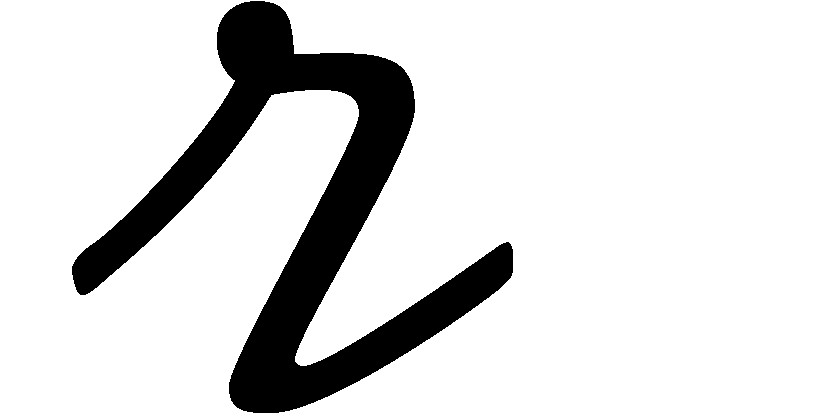
\includegraphics{ScriptR}}\!\!$}}}
\def\brcurs{{\mbox{$\resizebox{.16in}{.08in}{
\includegraphics{BoldR}}$}}}
\def\hrcurs{{\mbox{$\hat \brcurs$}}}
\newcommand{\fpe}{\dfrac{1}{4\pi\epsilon_0}}
\newcommand{\mfp}{ \dfrac{\mu_0}{4\pi} }
\newcommand{\wtRc}{\left[\omega(t-\rcurs/c)\right]}
\newcommand{\wtrc}{\left[\omega(t-r/c)\right]}
\begin{document}
	%\beamertemplatenavigationsymbolsempty
	\author{Karthik J\\(DP150006)}
	\title{Retarded Potentials due to an \\Oscillating Magnetic Dipole}
	\subtitle{\vspace{20pt}Semester 10\\PG.P.10.5 Classical Electrodynamics - II}
	%\logo{}
	%\institute{RIE Mysore}
	%\date{}
	%\subject{}
	%\setbeamercovered{transparent}
	%\setbeamertemplate{navigation symbols}{}
	\setbeamertemplate{itemize items}[default]
	\setbeamertemplate{enumerate items}[default]
	\metroset{numbering=none, progressbar = foot}
	\begin{frame}[plain]
		\maketitle
	\end{frame}
	
	\section{Introduction : \\Retarded Potentials}
	
	\begin{frame}
		{Maxwell's Equations}
		
		\begin{tcolorbox}
			\begin{eqnarray}
			\Div{E} &=& \dfrac{\rho}{\epsilon_0} \label{eqn : Max1} \\
			\Curl{E} &=& -\pdert{\vec{B}} \label{eqn : Max2}\\
			\Div{B} &=& 0 \label{eqn : Max3}\\
			\Curl{B} &=& \mu_0 \vec{J} + \mu_0 \epsilon_0 \pdert{\vec{E}} \label{eqn : Max4}
			\end{eqnarray}
		\end{tcolorbox}
	\end{frame}
	
	\begin{frame}%{The inhomogenous equation relating the potentials}
		%\small
		The four equations by Maxwell give rise to the formulation of a \za{scalar electric potential} $ V $ and a \za{vector magnetic potential} $ \vec{A} $. These potentials are related to the respective fields by
			
			\begin{equation}\label{eqn : E-field-pot}
				\vec{E} = -\vec{\nabla}V - \pdert{\vec{A}}
			\end{equation}
			
			\begin{equation}\label{eqn : B-field-pot}
			\vec{B} = \Curl{A}
			\end{equation}
			
	Using equations \ref{eqn : E-field-pot} and \ref{eqn : B-field-pot}, the four Maxwell's equations can be written into two coupled inhomogenous differential equations:
	\begin{equation}\label{eqn : inhomo-1}
		\Lap V + \pdert{ }\left(\Div{A}\right) = - \dfrac{\rho}{\epsilon_0}
	\end{equation}
	\begin{equation}\label{eqn : inhomo-2}
		\left( \Lap \vec{A} - \mu_0\epsilon_0 \pdertt{\vec{A}}\right)  - \vec{\nabla}\left( \Div{A} + \mu_0\epsilon_0 \pdert{V} \right) = -\mu_0 \vec{J}
	\end{equation}
	
	The above two equations  contain all the information in Maxwell’s equations.
	\end{frame}

	\begin{frame}{Gauge Transformations}
		For any scalar function $\lambda(\vec{r}, t)$, we can add $ \Grad\lambda $ to $\A$, provided we simultaneously subtract $ \left(\pdert{\lambda}\right) $ from $ V $. This will not affect the
		physical quantities $ \vec{E} $ and $ \vec{B} $. Such changes in $ V $ and $\A $ are called \za{gauge transformations}. \\
		\textit{i.e.,}
		\begin{eqnarray}
			\A' &=& \A + \Grad \lambda\\
			V'  &=& V - \pdert{\A}
		\end{eqnarray}
	\end{frame}

	\begin{frame}{Lorenz Gauge}
		In \za{Lorenz gauge}, we pick:
		\begin{equation}\label{eqn : Lorenz-gauge}
			\Div{A} = -\mu_0\epsilon_0 \pdert{V}
		\end{equation}
		From equation (\ref{eqn : inhomo-2}),
		\[ \left( \Lap \vec{A} - \mu_0\epsilon_0 \pdertt{\vec{A}}\right)  - \vec{\nabla}\left( \Div{A} + \mu_0\epsilon_0 \pdert{V} \right) = -\mu_0 \vec{J} \]
		Applying the gauge condition the two coupled inhomogenous equations reduce to a much simpler \textit{symmetric} form,
		\begin{eqnarray}
			\Lap \A - \mu_0\epsilon_0 \pdertt{\A} &=& -\mu_0\J\\
			\Lap V - \mu_0\epsilon_0 \pdertt{V} &=& -\dfrac{\rho}{\epsilon_0}
		\end{eqnarray}
	\end{frame}

	\begin{frame}
		\small
			\[\Lap \A - \mu_0\epsilon_0 \pdertt{\A} = -\mu_0\J\]
			\[\Lap V - \mu_0\epsilon_0 \pdertt{V} = -\dfrac{\rho}{\epsilon_0}\]
			\pause
			In the static case, these equations reduce to the Poisson's equations \pause
			\[\Lap \A = -\mu_0\J\]
			\[\Lap V = -\dfrac{\rho}{\epsilon_0}\]
			\pause
			\hrule
			\begin{columns}
				\column{0.5\textwidth}
				\begin{figure}[!htb]
					\centering
					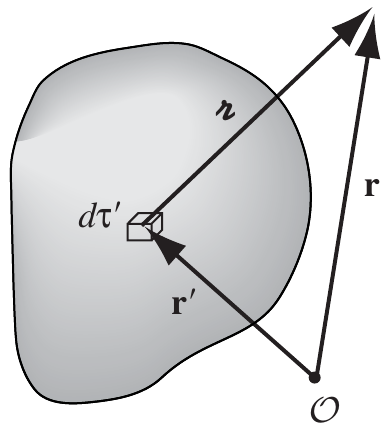
\includegraphics[scale=0.25]{vectors}
				\end{figure}
			\pause	
				\column[c]{0.5\textwidth}
			The solutions of the Poisson's equations are:
			\[ V(\vec{r}) = \fpe \int \dfrac{\rho(\vec{r'})}{\rcurs} \, d\tau' \]
			\[ \A(\vec{r}) = \mfp \int \dfrac{\J(\vec{r'})}{\rcurs} \, d\tau' \]
\end{columns}
	\end{frame}
	
	\begin{frame}
		The same general solution holds true for non-static sources as well;
		\begin{eqnarray}
			V(\vec{r}, t) &=& \fpe \int \dfrac{\rho(\vec{r'},t_r)}{\rcurs}\, d\tau' \label{eqn : ret-V}\\
			\A(\vec{r}, t) &=& \mfp \int \dfrac{\J(\vec{r'},t_r)}{\rcurs}\, d\tau' \label{eqn : ret-A}
		\end{eqnarray}
		\begin{itemize}
			\item 		In the non-static case, it’s not the status of the source \emph{right now} that matters, but its condition at some \emph{earlier time} $t_r$ (called the \za{retarded time}) when the
			``message'' left. Since this message must travel a distance  \rcurs (with a \emph{finite} speed $ c $), the delay is $\left( \dfrac{\rcurs}{c} \right)$ :
			\[ t_r \equiv t - \dfrac{\rcurs}{c} \]
			
			\item 		Here $\rho (\vec{r'} , t_r)$ is the charge density that prevailed at point $\vec{r'}$ at the retarded time $t_r$. Because the integrands are evaluated at the retarded time, these are called \za{retarded potentials}. 
		\end{itemize}
	\end{frame}
	
	\section{Retarded Potentials of a Magnetic Dipole}
	
	\begin{frame}
		\small
		\begin{columns}
			\column{0.5\textwidth}
			\begin{figure}[!htb]
				\centering
				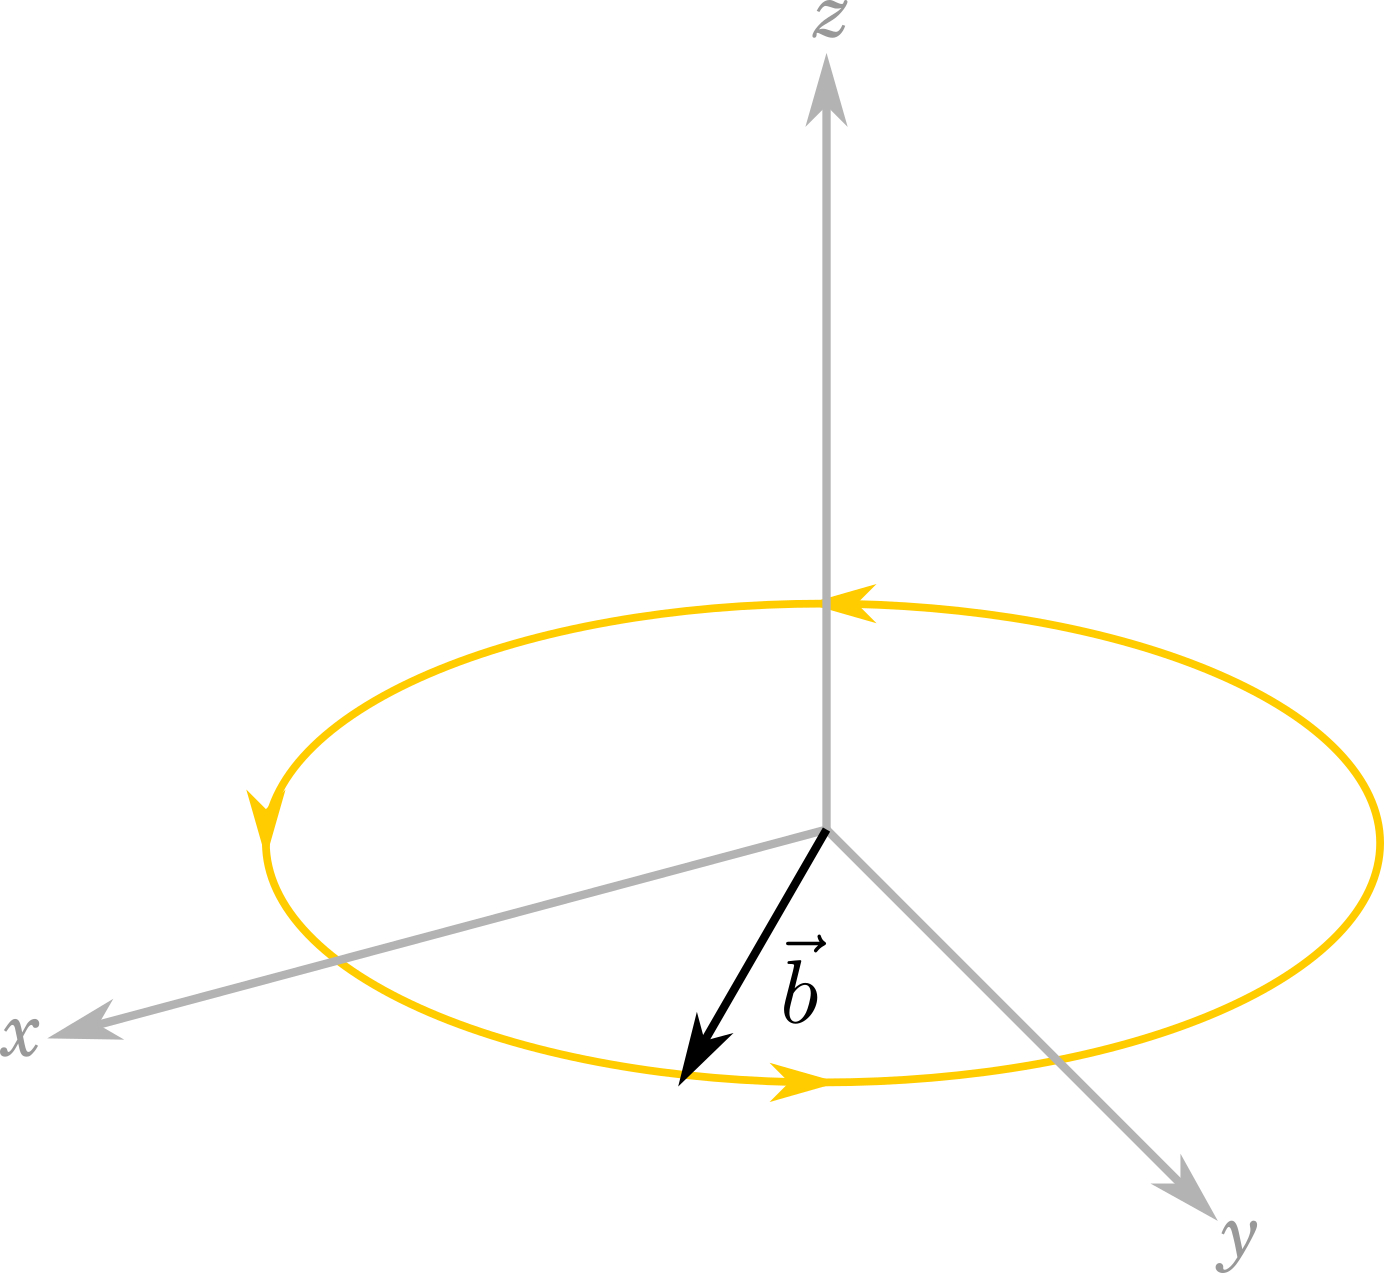
\includegraphics[scale=0.5]{dip-1}
			\end{figure}
			\column{0.5\textwidth}
			Consider a wire loop of radius $b$, around which an alternating current is flowing:
			\[ I(t) = I_0\, \cos(\omega t) \]
			\pause
			The \za{magnetic dipole moment} is given by
			\begin{dmath}
				\vec{m}(t) = I(t)\, \vec{a} = 	I(t) \pi b^2\, \hat{z} \pause
				= I_0\, \cos(\omega t) \pi b^2\, \hat{z} \pause
				= m_0 \, \cos(\omega t)\, \hat{z} \pause
			\end{dmath}
			where $ m_0 \equiv \pi b^2 I_0 $ is the maximum value of the magnetic dipole moment.\\
			\pause
			The loop is electrically neutral, so the electric potential
			\begin{tcolorbox}[colframe=amber, colback = amber!20]
				\begin{equation}\label{eqn : V}
					V = 0
				\end{equation}
			\end{tcolorbox}
		\end{columns}
		
	\end{frame}

	\begin{frame}
		\begin{figure}[!htb]
			\centering
			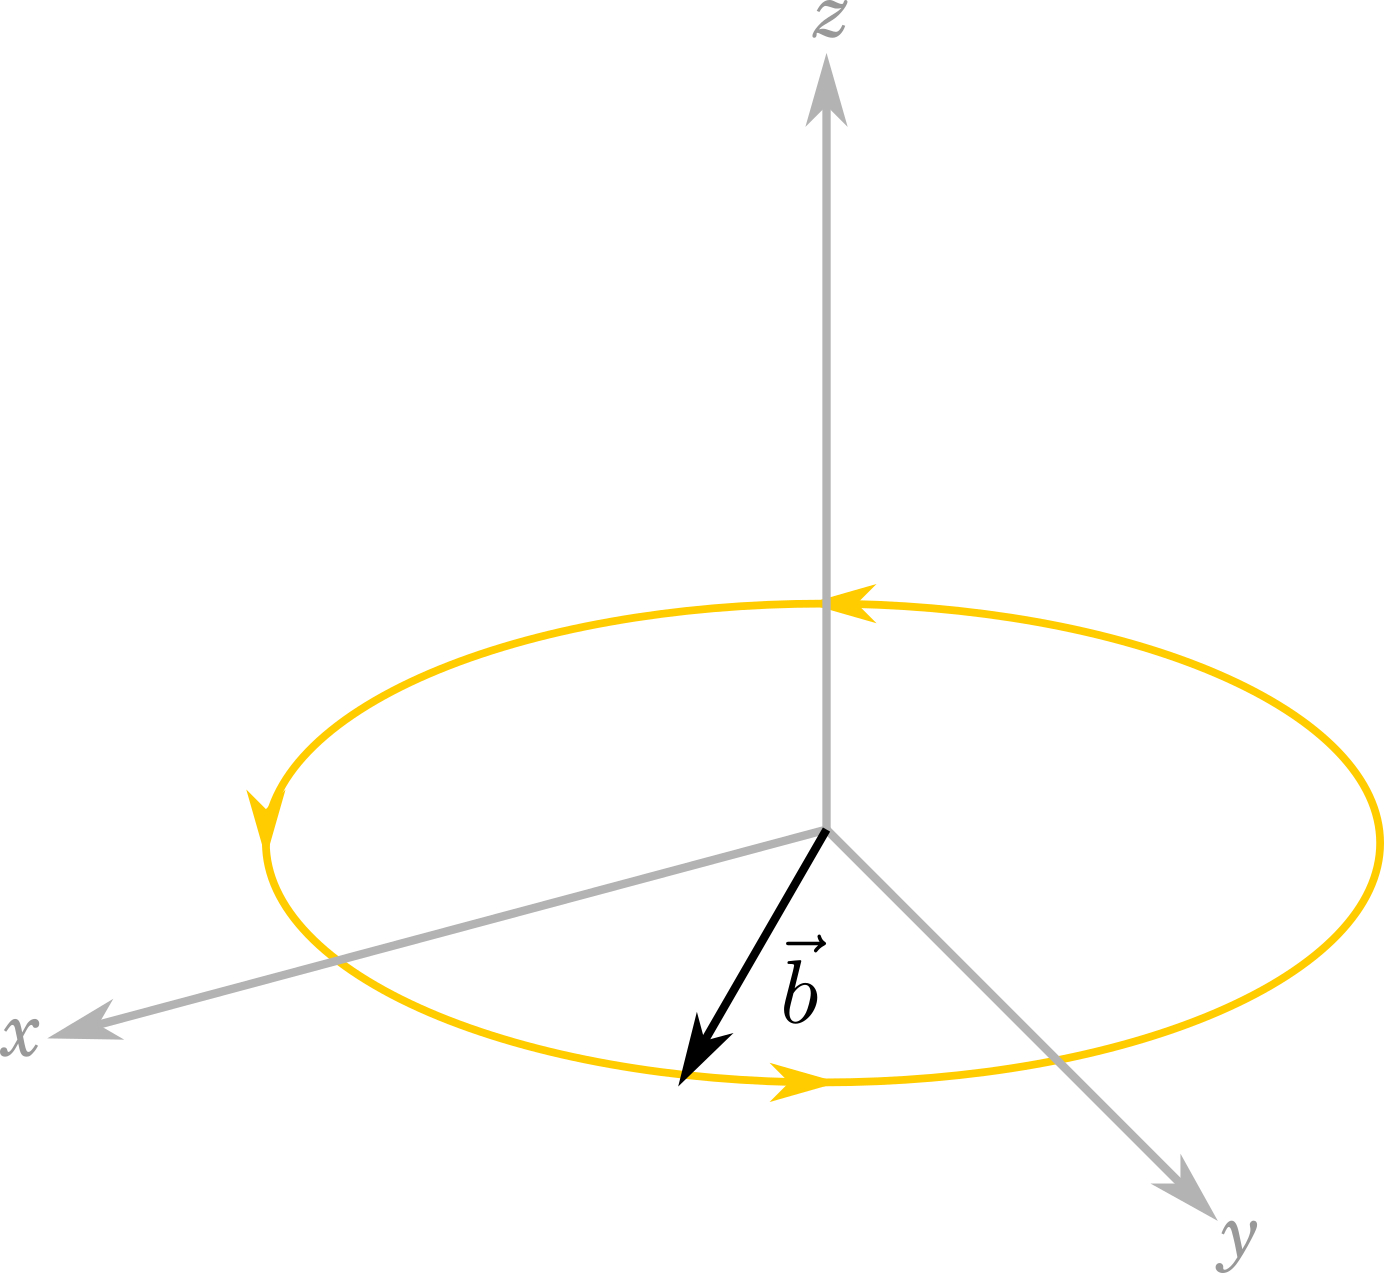
\includegraphics[scale=0.6]{dip-1}
		\end{figure}
	\end{frame}

	\begin{frame}
		\begin{figure}[!htb]
			\centering
			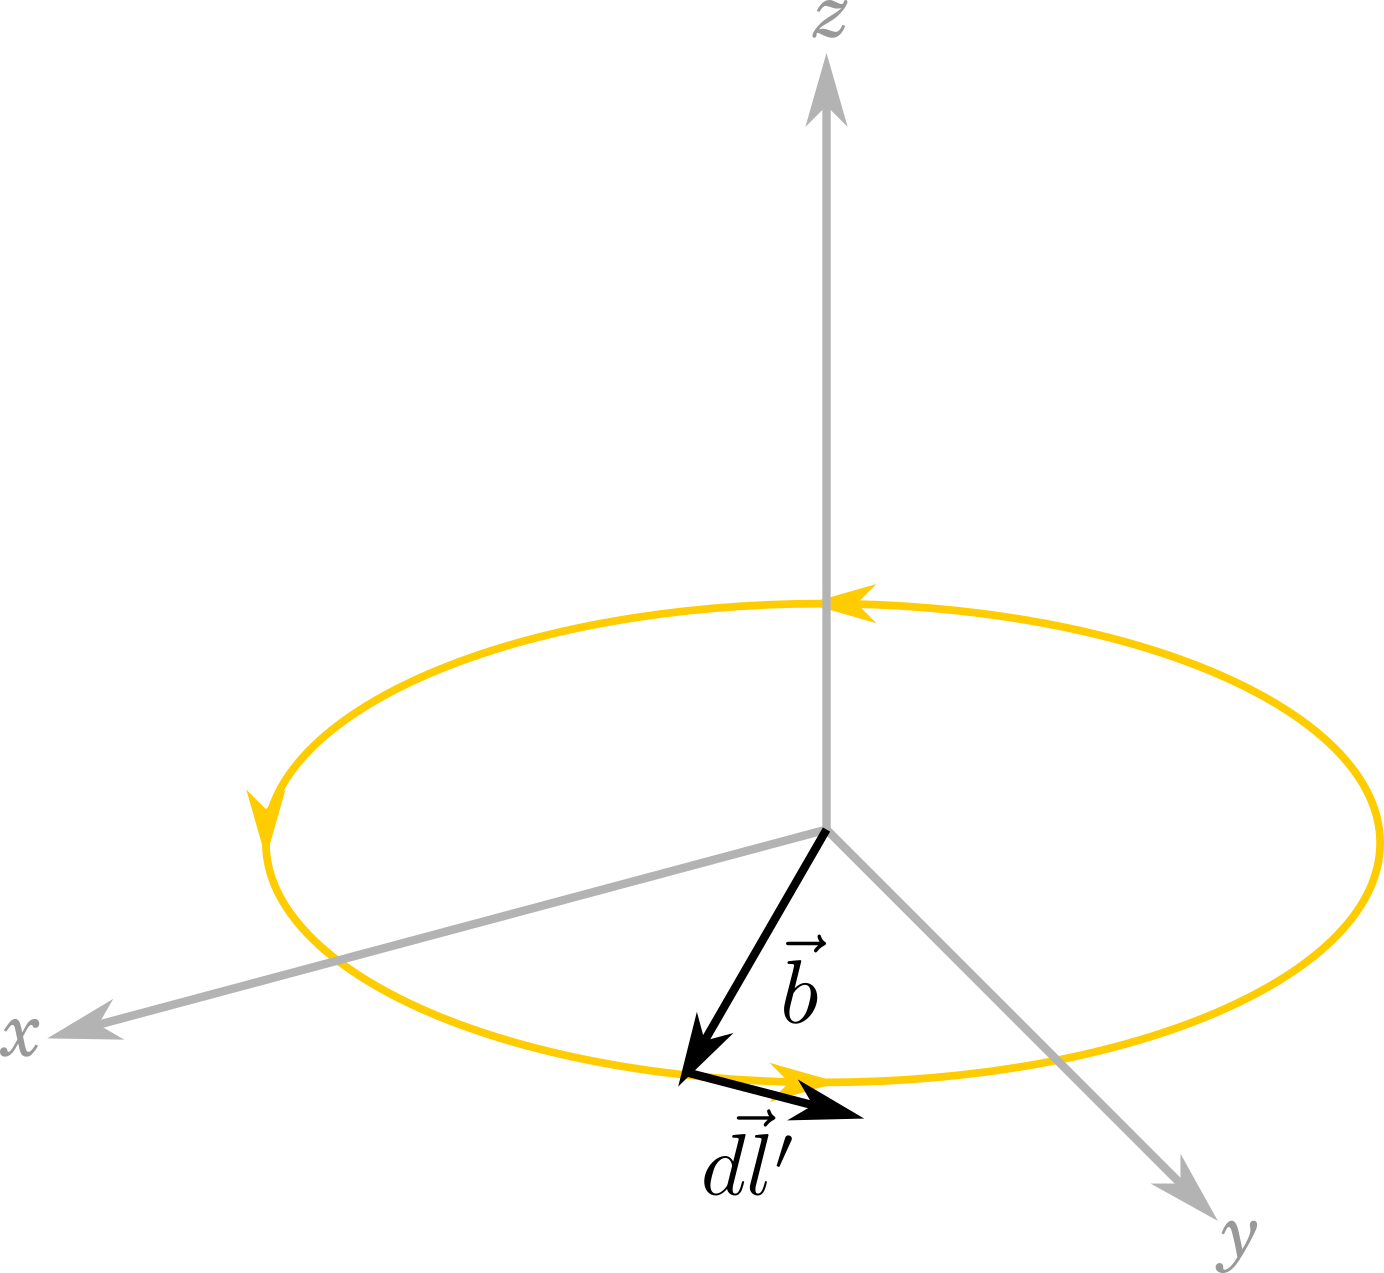
\includegraphics[scale=0.6]{dip-2}
		\end{figure}
	\end{frame}
	
	\begin{frame}
		\begin{figure}[!htb]
			\centering
			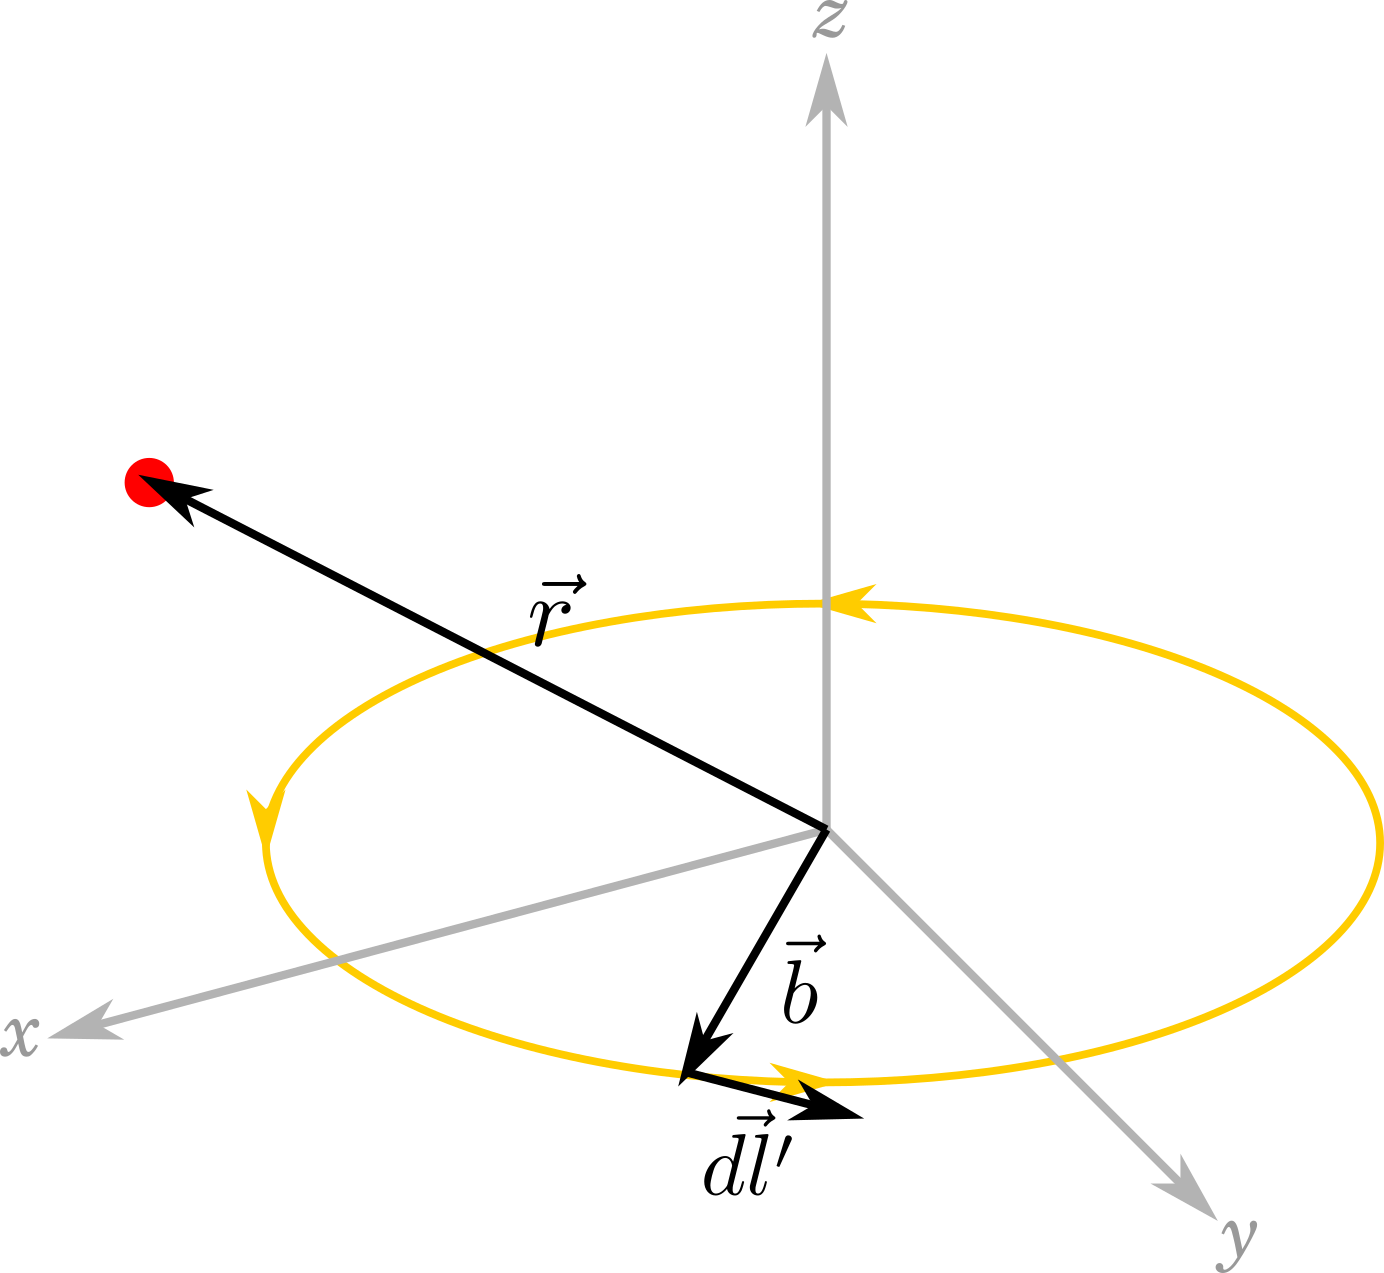
\includegraphics[scale=0.6]{dip-3}
		\end{figure}
	\end{frame}
	
	\begin{frame}
		\begin{figure}[!htb]
			\centering
			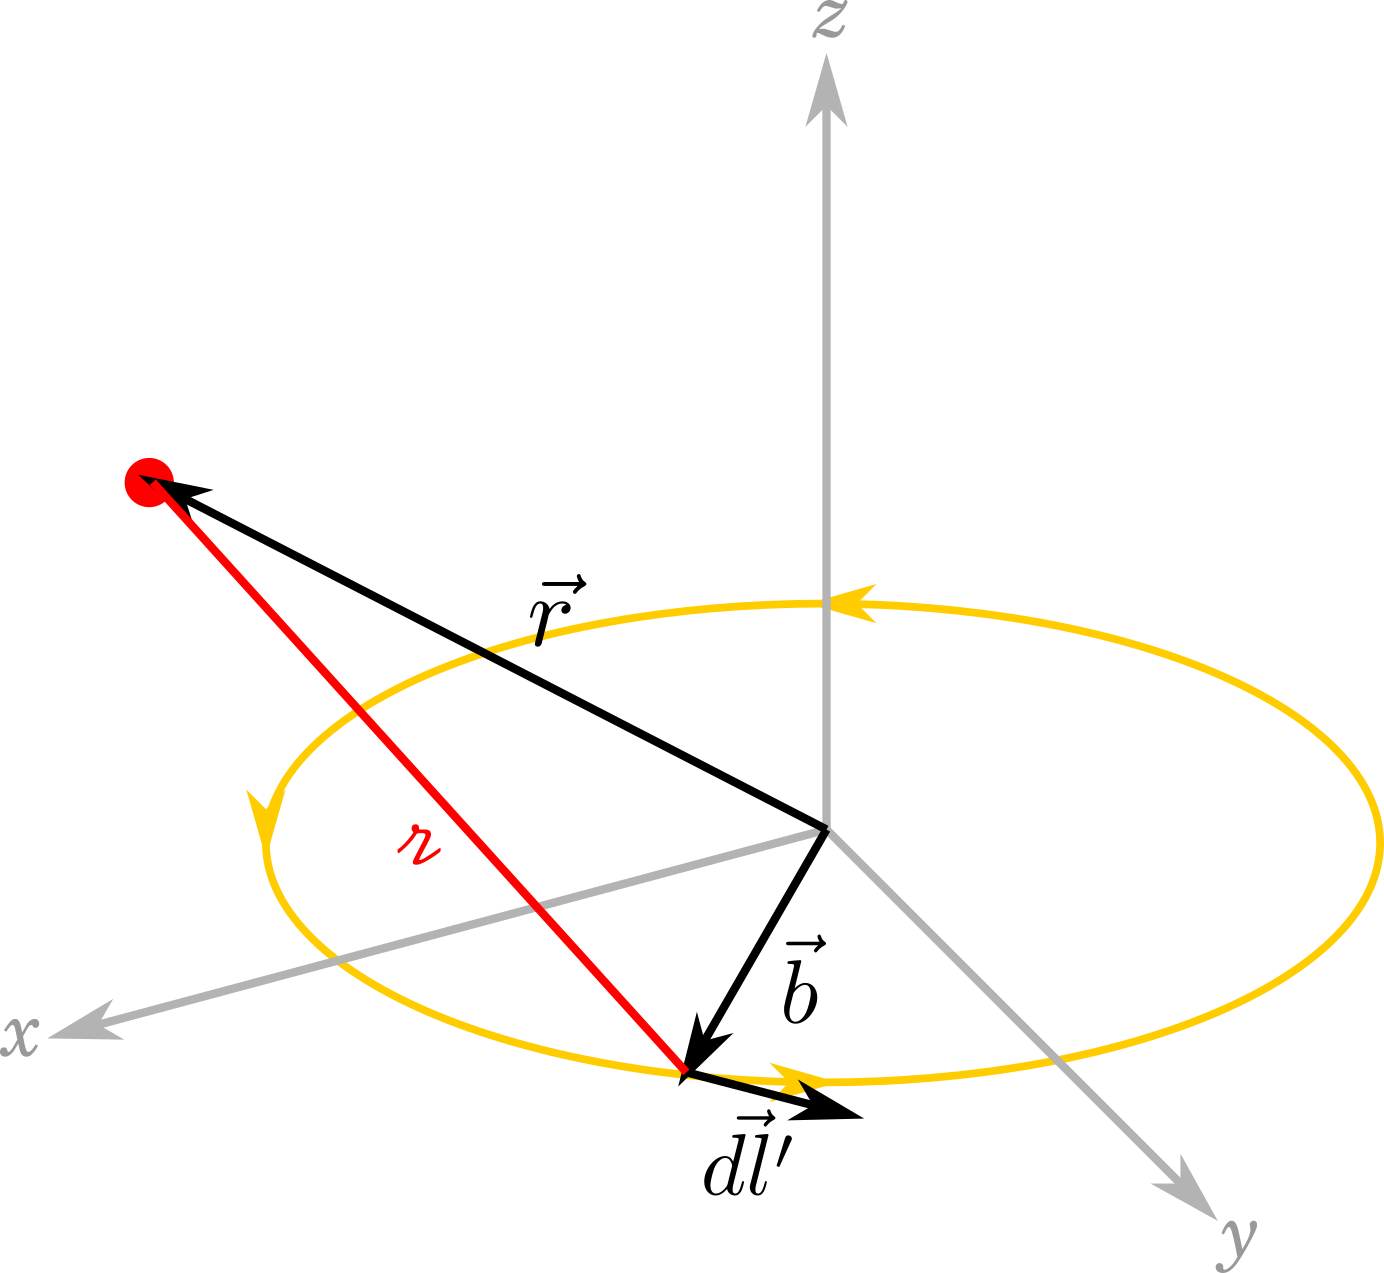
\includegraphics[scale=0.6]{dip-4}
		\end{figure}
	\end{frame}

	\begin{frame}
	\begin{columns}
		\column{0.5\textwidth}
				\begin{figure}[!htb]
			\centering
			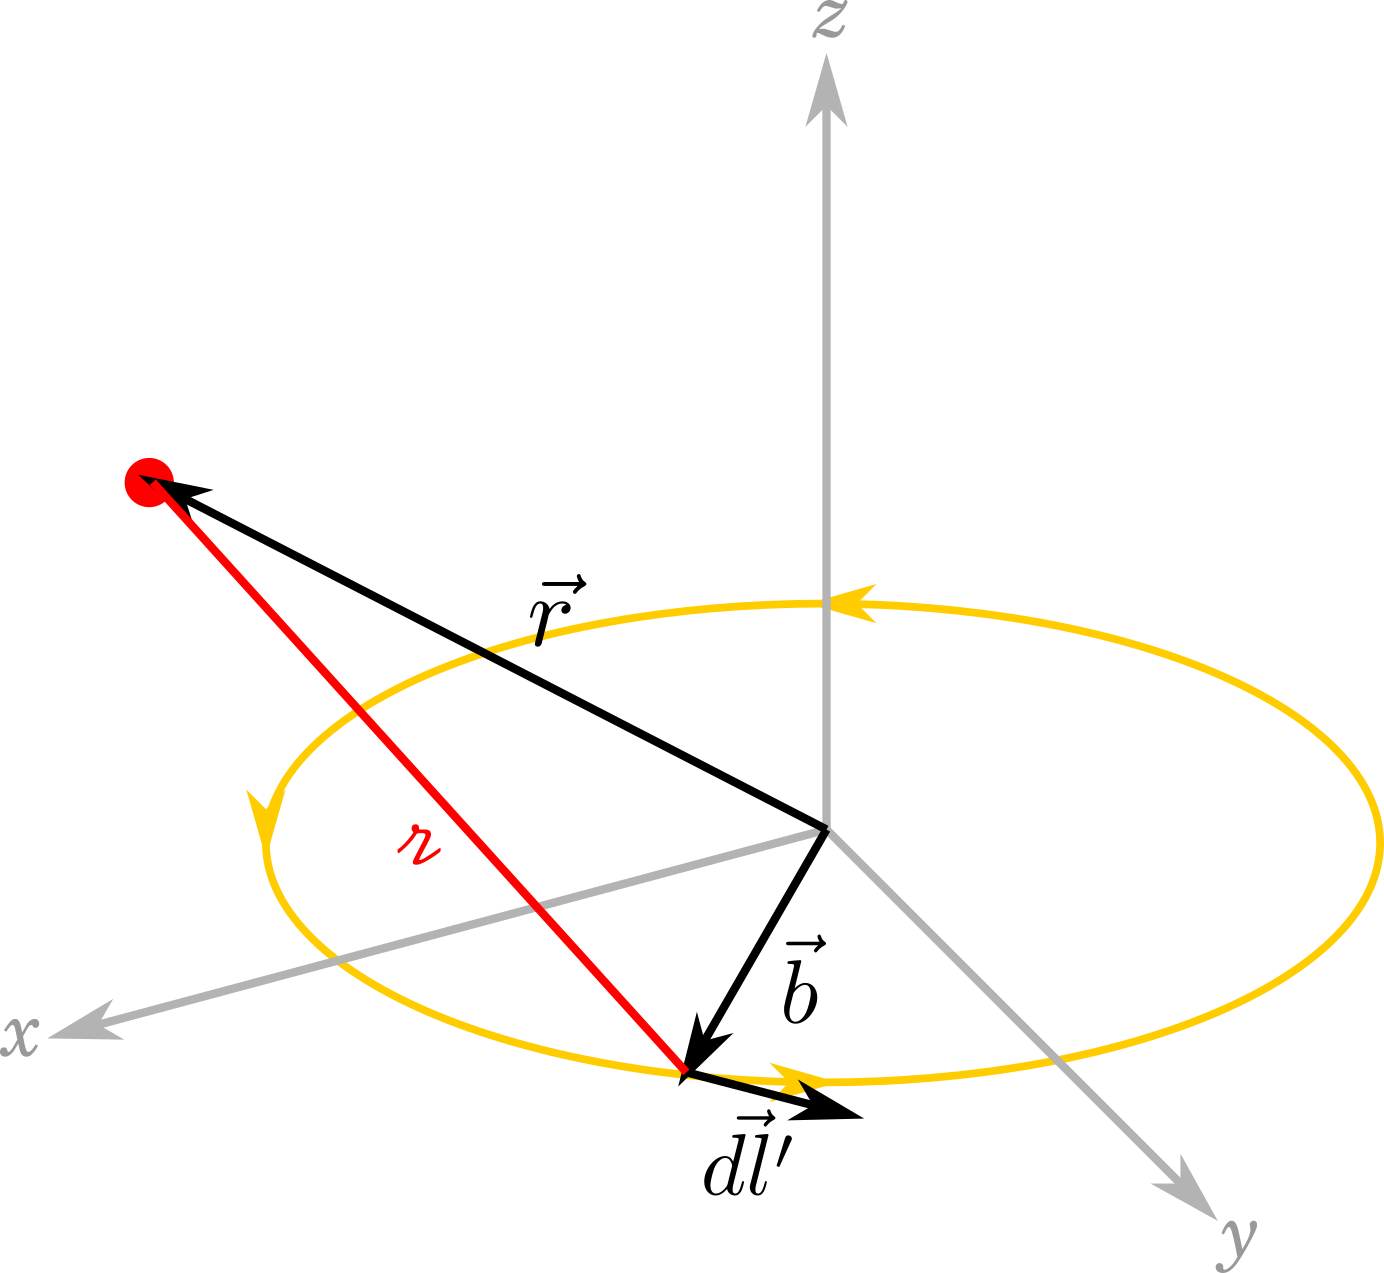
\includegraphics[scale=0.5]{dip-4}
		\end{figure}
		
		\column{0.5\textwidth}
		\pause
		The general equation for retarded magnetic potential (equation (\ref{eqn : ret-A})) is, \pause
		\[ \A(\vec{r}, t) = \mfp \int \dfrac{\J(\vec{r'},t_r)}{\rcurs}\, d\tau' \]\pause
		\begin{dmath*}
			\A(\vec{r}, t) = \mfp \int \dfrac{I(t_r)}{\rcurs}\, \vec{dl'} \pause
			=\mfp \int \dfrac{I_0 \cos (\omega t_r)}{\rcurs}\, \vec{dl'} \pause
			= \mfp \int \dfrac{I_0 \cos \left[\omega \left( t - \rcurs/c \right)  \right]}{\rcurs}\, \vec{dl'} 
		\end{dmath*}
	\end{columns}
	\end{frame}
	
	\begin{frame}
		\begin{columns}
			\column[]{0.5\textwidth}
			\begin{figure}[!htb]
				\centering
				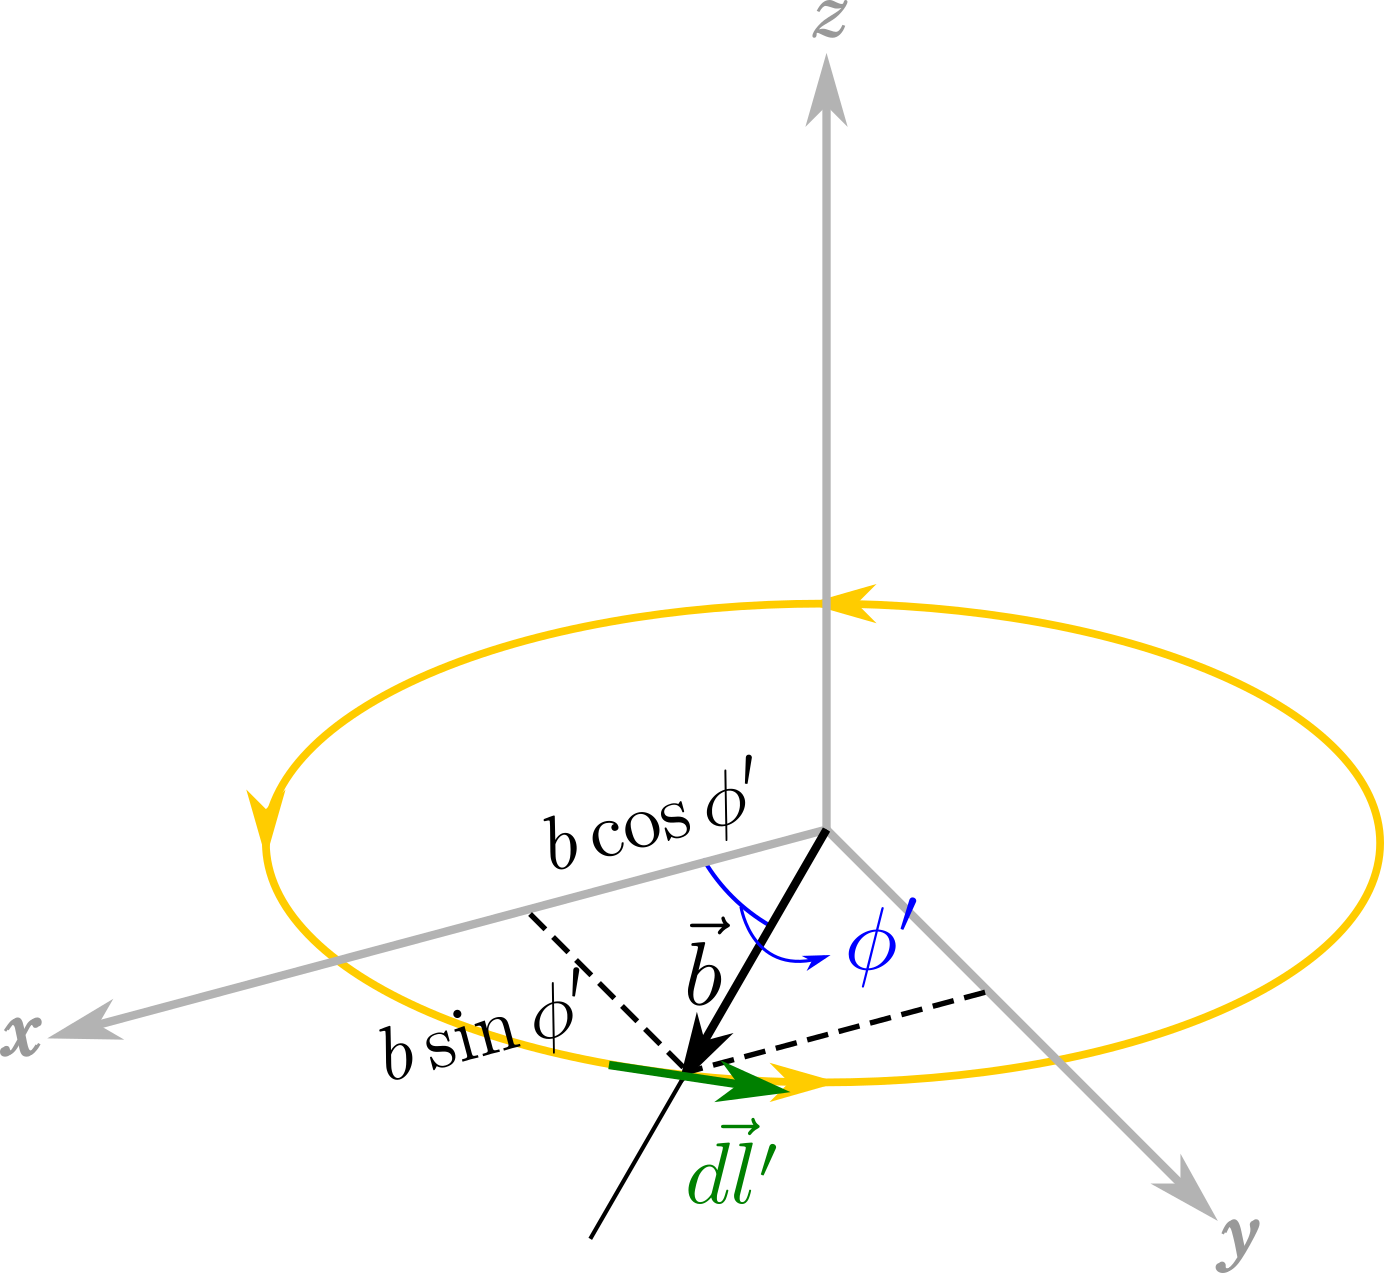
\includegraphics[scale=0.5]{b-components-dl}
			\end{figure}
			\column[]{0.5\textwidth}
			\pause
			\[ \vec{dl} = dx\, \hat{x} + dy\, \hat{y} + dz\, \hat{z} \]
			\pause
			For the source co-ordinates,\pause
			\begin{align*}
				x' =& b\cos\phi' & \implies dx' =& -b\sin\phi'\, d\phi' \\
				y' =& b\sin\phi' & \implies dy' =&\ b\cos\phi'\, d\phi'\\
				z' =& 0 & \implies dz' = &\ 0  
			\end{align*}
			\pause
			\begin{dmath*}
				\vec{dl'} = dx'\, \hat{x} + dy'\, \hat{y} + dz'\, \hat{z}  
				=  -b\sin\phi'\, d\phi' \, \hat{x} + b\cos\phi'\, d\phi' \, \hat{y}
			\end{dmath*}
		\end{columns}
	\end{frame}

	\begin{frame}
		\begin{columns}
			\column[]{0.5\textwidth}
			Consider a point on the xz plane.
			
\begin{figure}
	\centering
	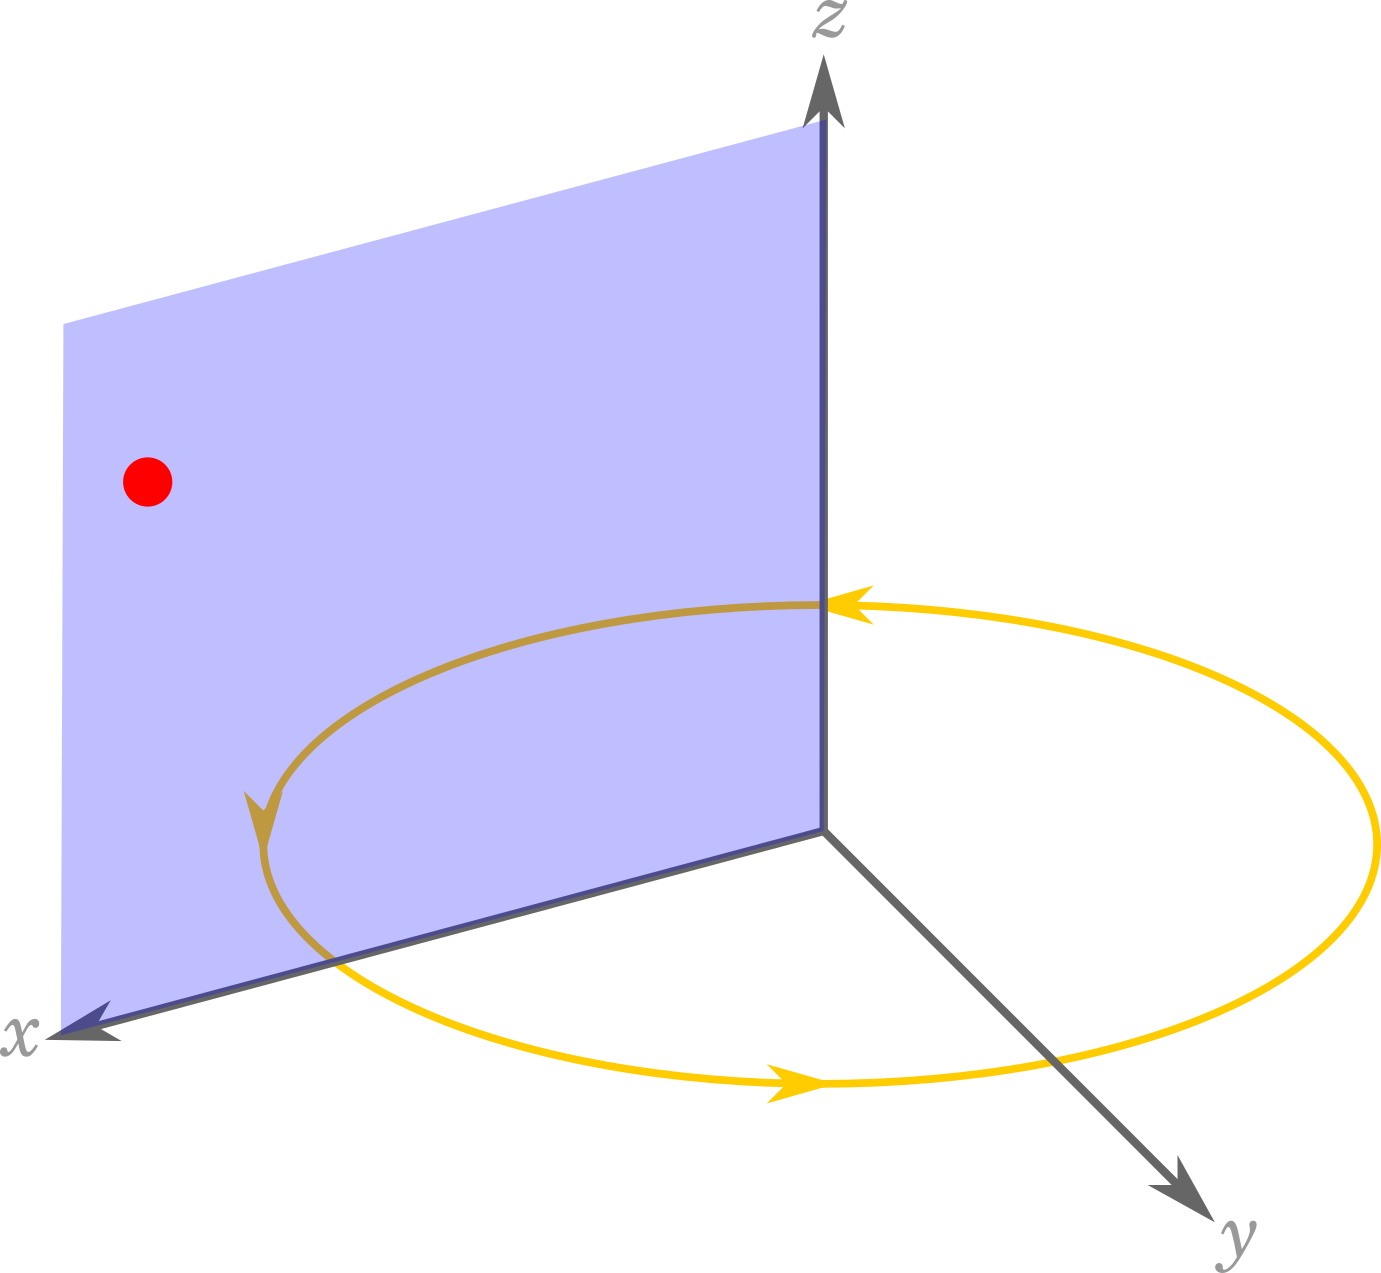
\includegraphics[width=0.7\linewidth]{dip-point-plane}
	\label{fig:dip-point-plane}
\end{figure}
			\column[]{0.5\textwidth}
			
			
		\end{columns}
	\end{frame}

\begin{frame}
	\begin{columns}
		\column[]{0.5\textwidth}
		Consider a point on the xz plane.
		
		\begin{figure}
			\centering
			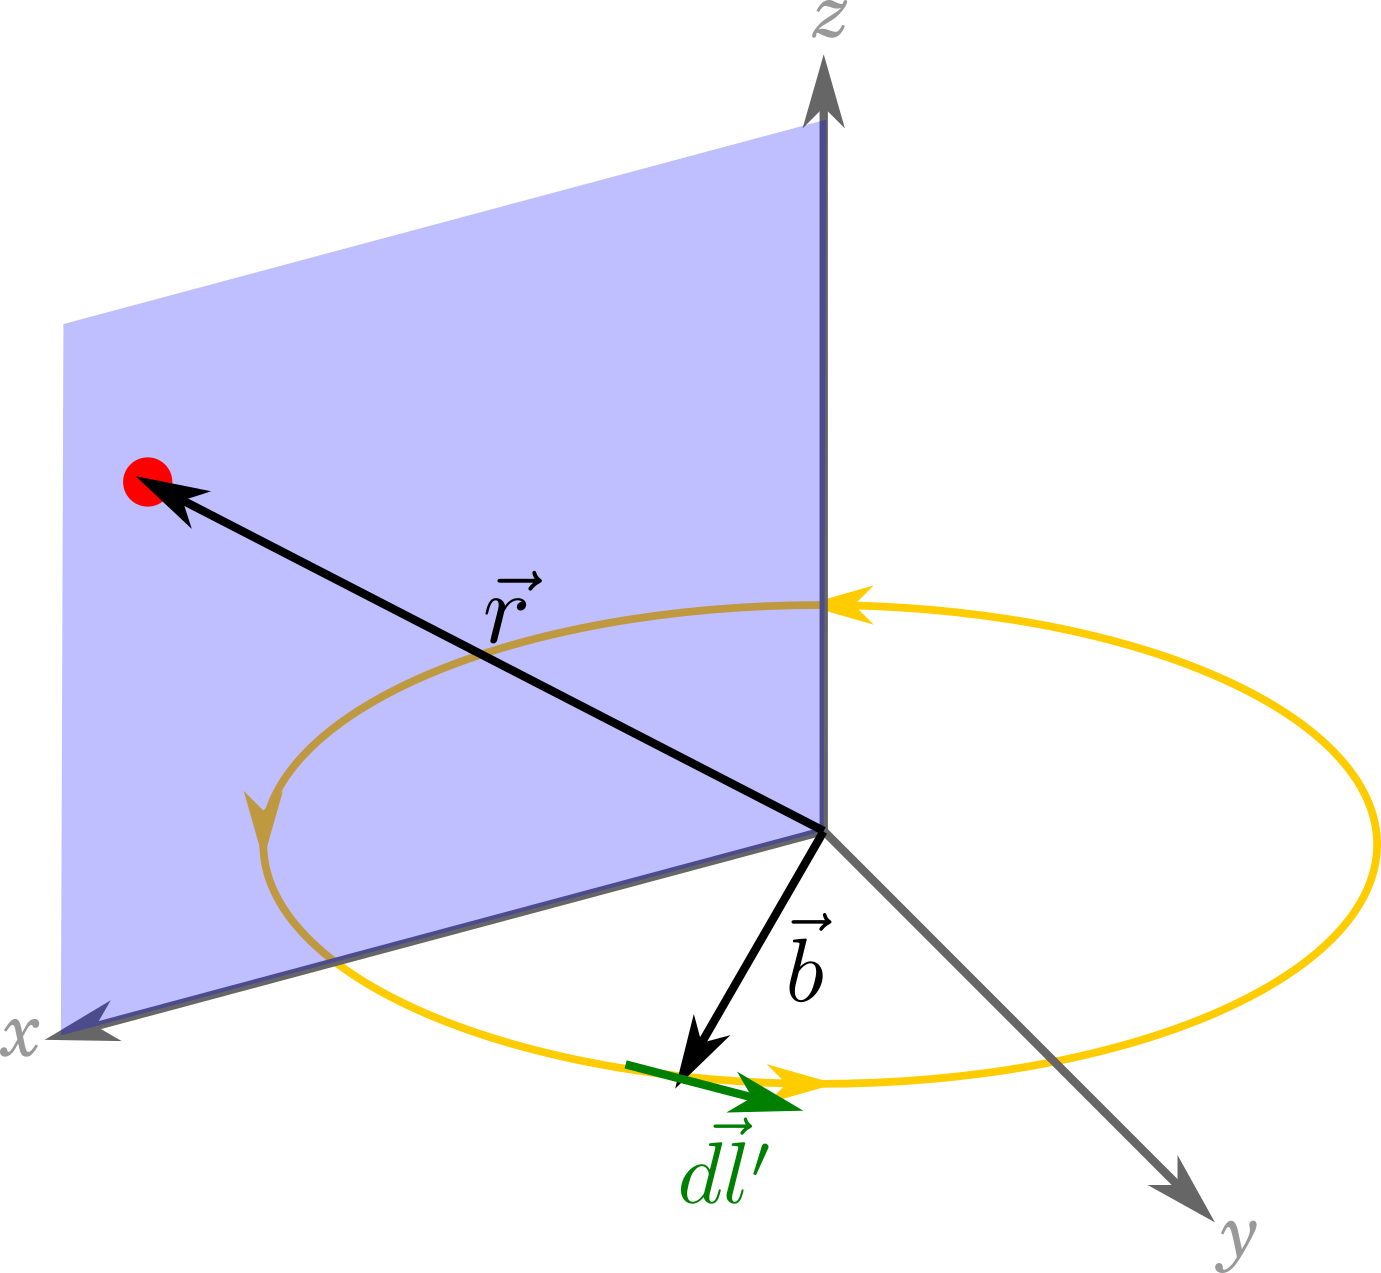
\includegraphics[width=0.7\linewidth]{dip-point-plane-2}
			\label{fig:dip-point-plane-2}
		\end{figure}
		\column[]{0.5\textwidth}
		
	\end{columns}
\end{frame}

\begin{frame}
	\begin{columns}
		\column[]{0.5\textwidth}
		Consider a point on the xz plane.
		
		\begin{figure}
			\centering
			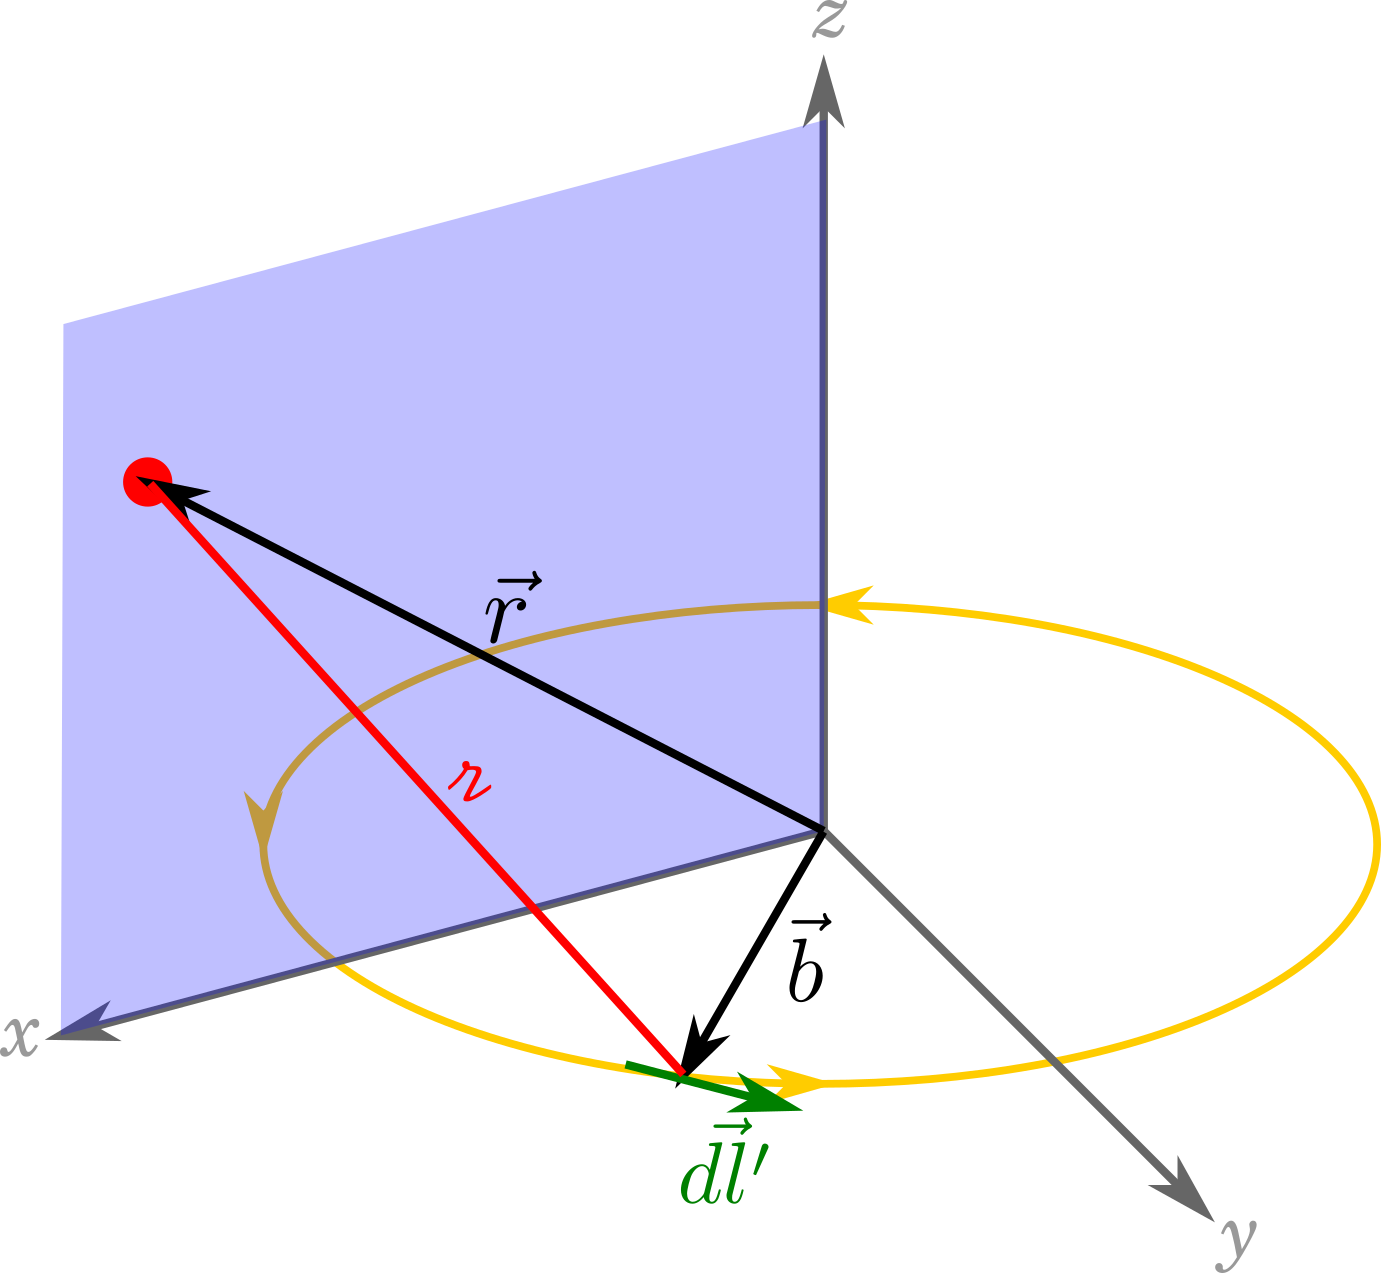
\includegraphics[width=0.7\linewidth]{dip-point-plane-3}
			\label{fig:dip-point-plane-3}
		\end{figure}
		\column[]{0.5\textwidth}
		
		\[ \vec{A}(\vec{r},t) = \mfp \int \dfrac{I_0 \cos \left[\omega \left( t - \rcurs/c \right) \right]}{\rcurs}\, \vec{dl'} \]
		
	\end{columns}
\end{frame}

\begin{frame}
	\begin{columns}
		\column[]{0.5\textwidth}
		Consider a point on the xz plane.
		
		\begin{figure}
			\centering
			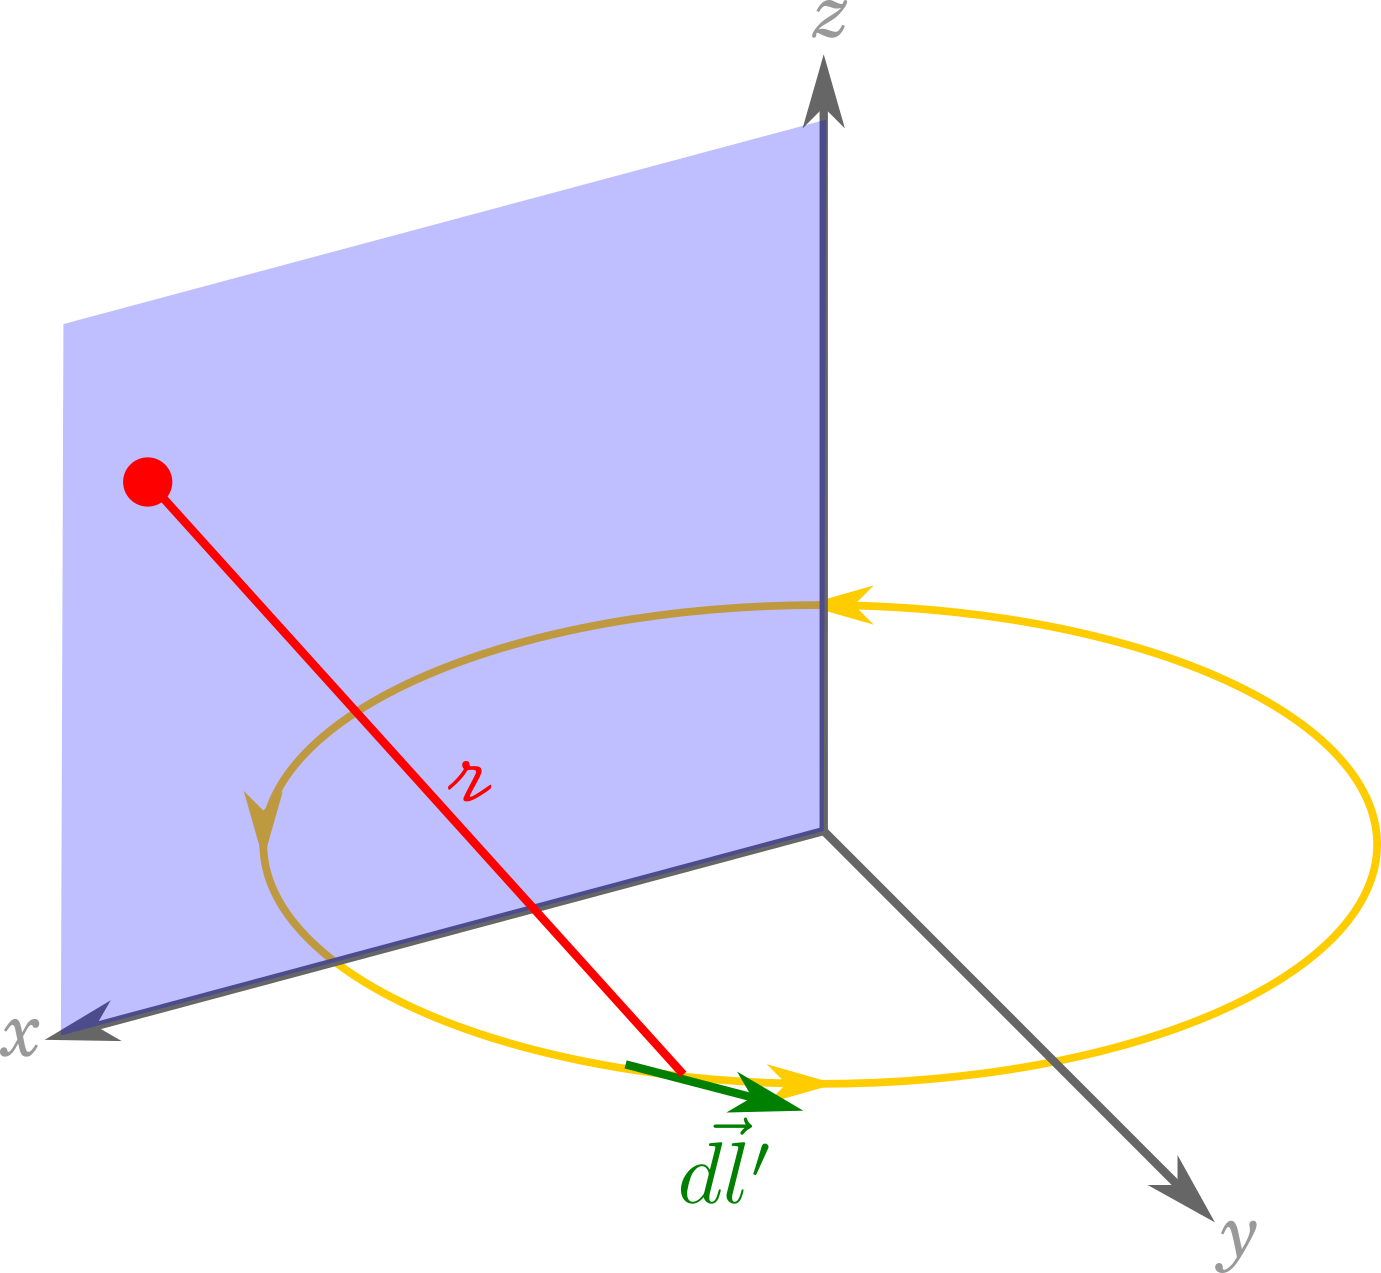
\includegraphics[width=0.7\linewidth]{dip-point-plane-4}
			\label{fig:dip-point-plane-4}
		\end{figure}
		\column[]{0.5\textwidth}
		
		\[ \vec{A}(\vec{r},t) = \mfp \int \dfrac{I_0 \cos \left[\omega \left( t - \rcurs/c \right) \right]}{\rcurs}\, \vec{dl'} \]
		
	\end{columns}
\end{frame}

\begin{frame}
	\begin{columns}
		\column[]{0.5\textwidth}
		Consider a point on the xz plane.
		
		\begin{figure}
			\centering
			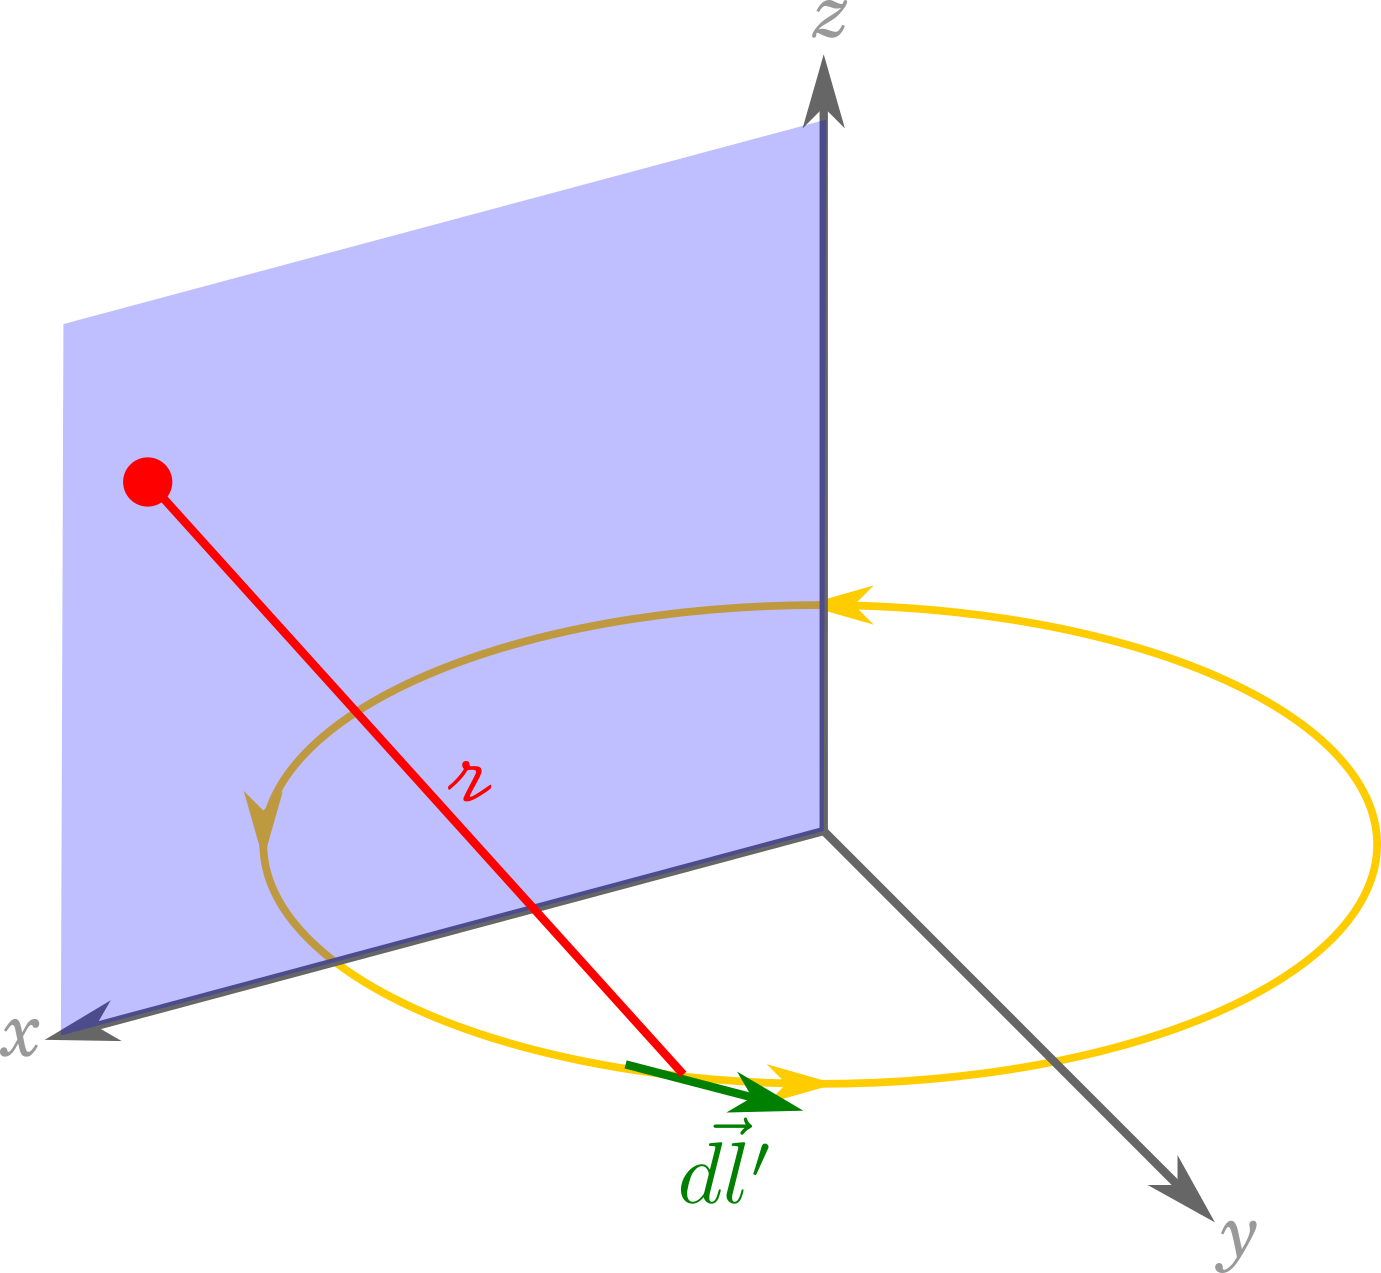
\includegraphics[width=0.7\linewidth]{dip-point-plane-4}
			\label{fig:dip-point-plane-4}
		\end{figure}
		\column[]{0.5\textwidth}
		
		\[ \vec{A}(\vec{r},t) = \mfp \int \dfrac{I_0 \cos \left[\omega \left( t - \rcurs/c \right) \right]}{\rcurs}\, \color{high}{\vec{dl'}} \]
		
	\end{columns}
\end{frame}

\begin{frame}
	\begin{columns}
		\column[]{0.5\textwidth}
		Consider a point on the xz plane.
		
		\begin{figure}
			\centering
			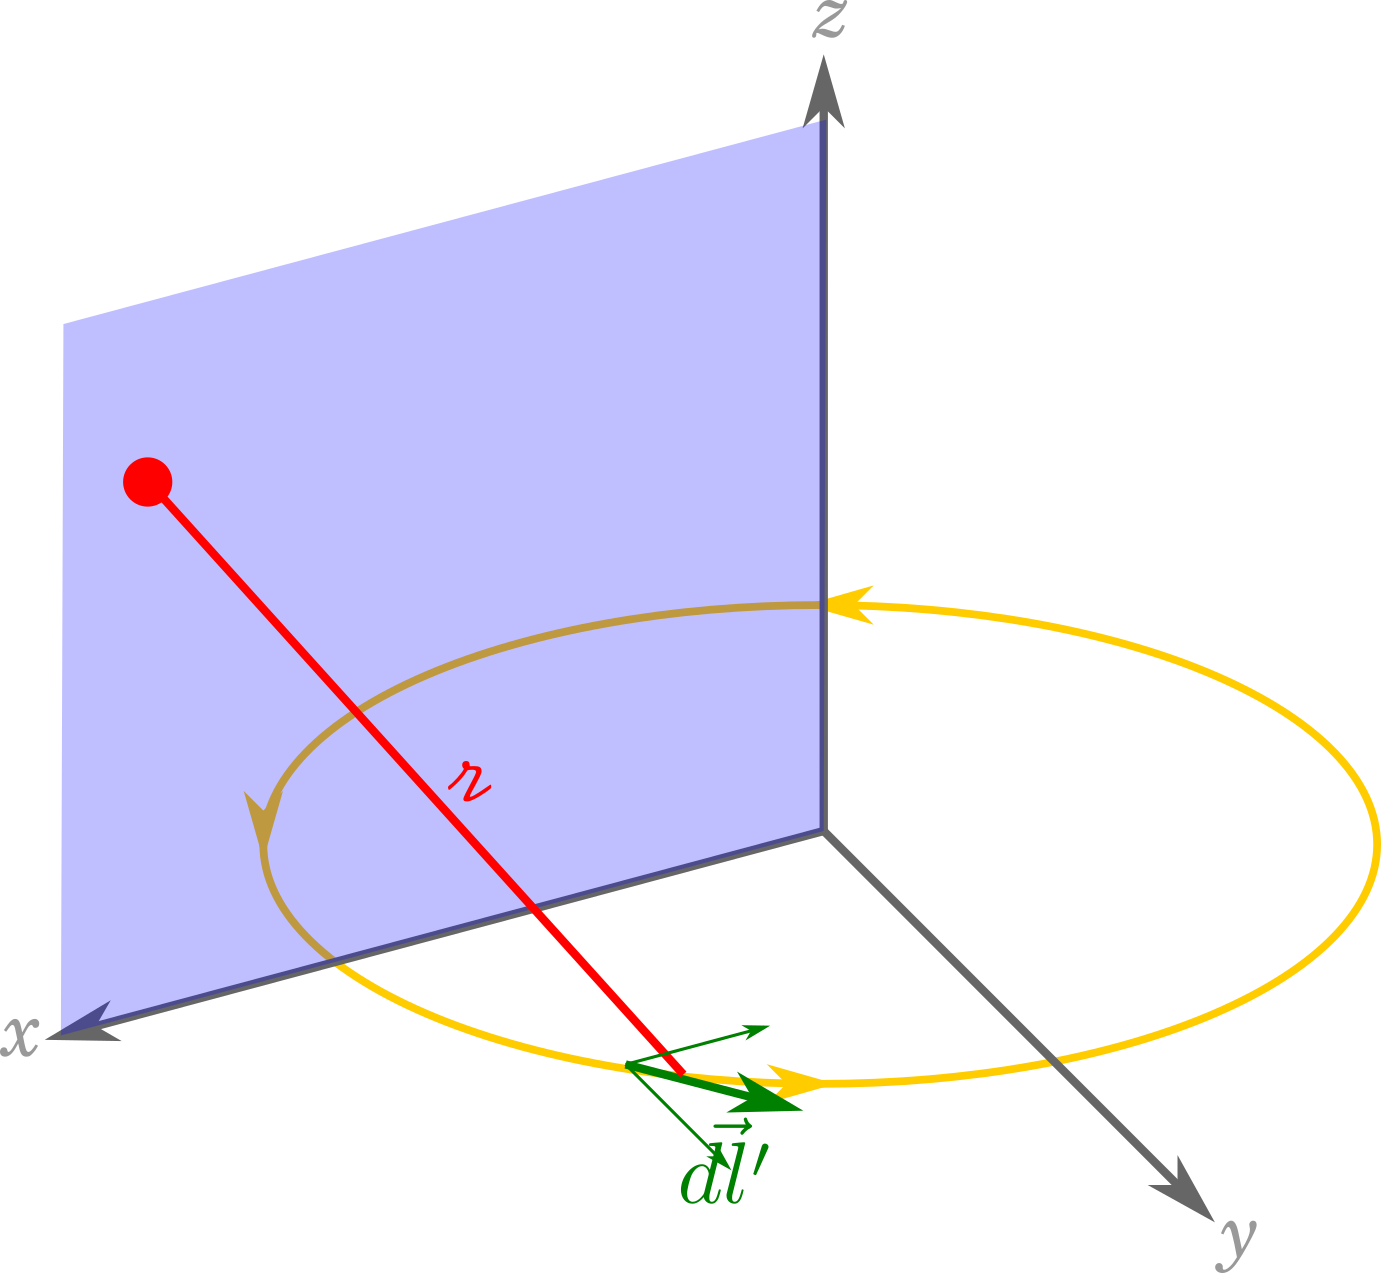
\includegraphics[width=0.7\linewidth]{dip-point-plane-5}
			\label{fig:dip-point-plane-5}
		\end{figure}
		\column[]{0.5\textwidth}
		
		\[ \vec{A}(\vec{r},t) = \mfp \int \dfrac{I_0 \cos \left[\omega \left( t - \rcurs/c \right) \right]}{\rcurs}\, \color{high}{\vec{dl'}} \]
		
	\end{columns}
\end{frame}

\begin{frame}
	\begin{columns}
		\column[]{0.5\textwidth}
		Consider a point on the xz plane.
		
		\begin{figure}
			\centering
			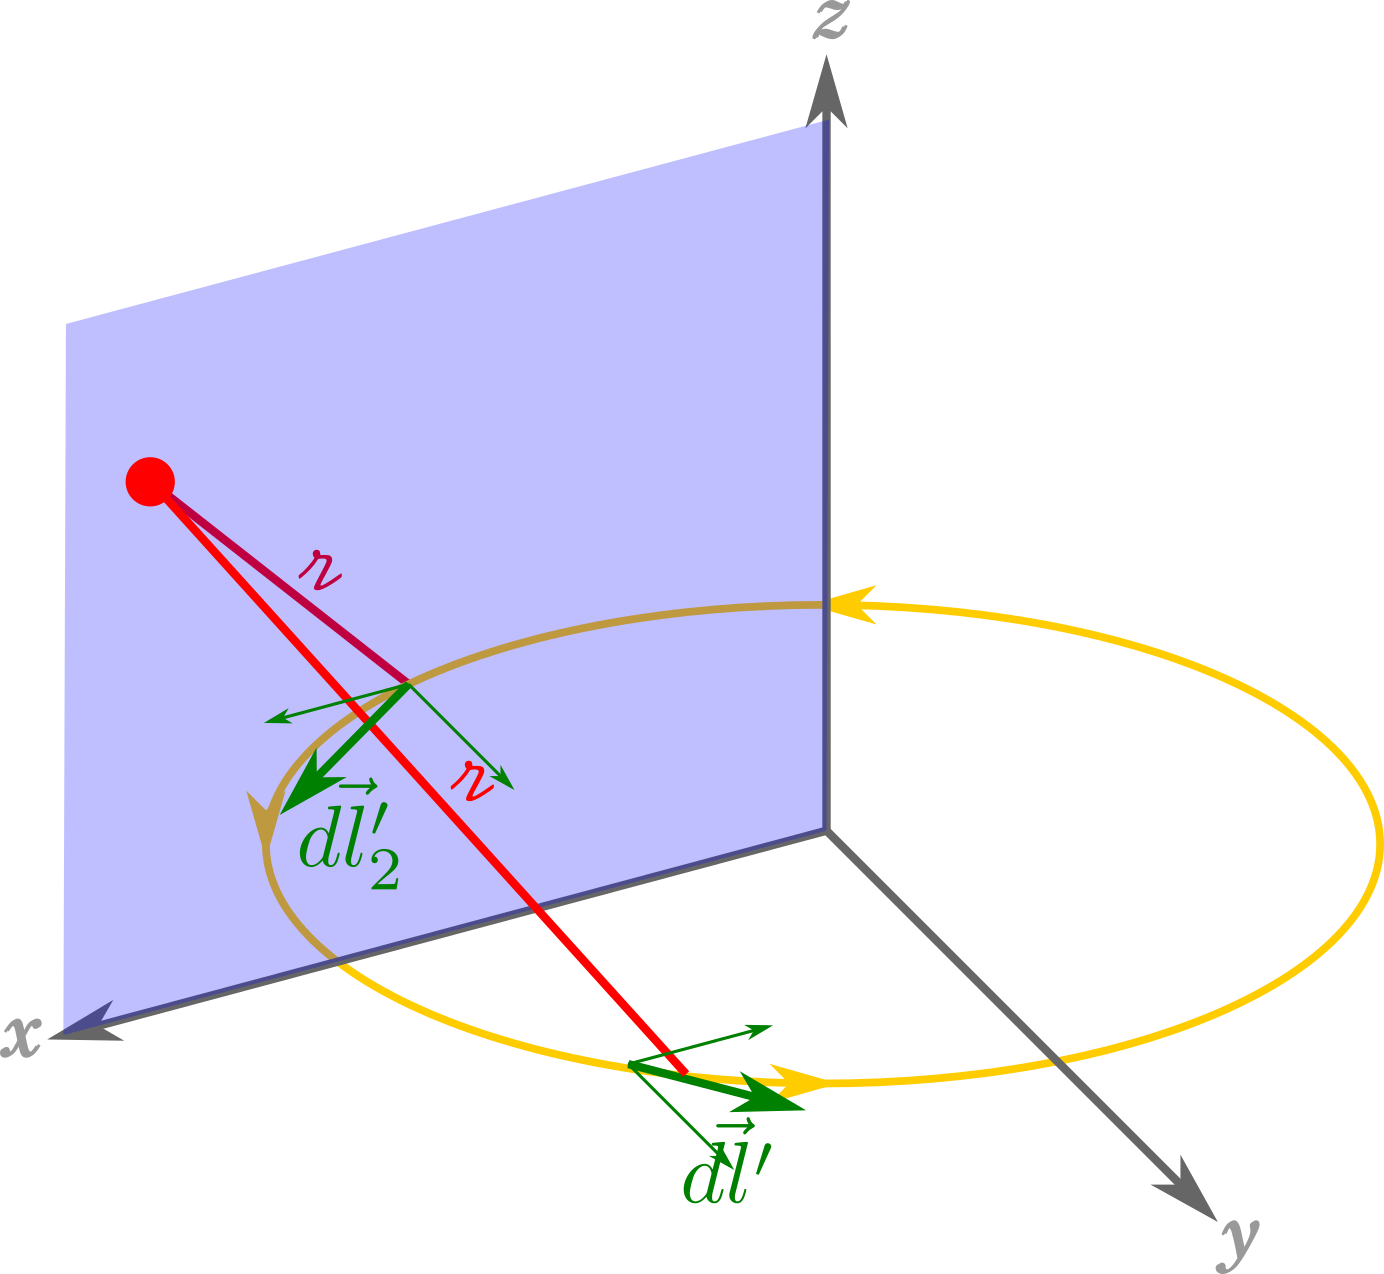
\includegraphics[width=0.7\linewidth]{dip-point-plane-6}
			\label{fig:dip-point-plane-6}
		\end{figure}
		\column[]{0.5\textwidth}
		
		\[ \vec{A}(\vec{r},t) = \mfp \int \dfrac{I_0 \cos \left[\omega \left( t - \rcurs/c \right) \right]}{\rcurs}\, \vec{dl'} \]
			\pause
		Hence, $ \vec{A} $ has $ \hat{y} $-component only.
		\pause
		\[ \vec{dl'} = -b\sin\phi'\, d\phi' \, \hat{x} + b\cos\phi'\, d\phi' \, \hat{y} \]%
		\pause%
		\[ \therefore \vec{dl'} = b\cos\phi'\, d\phi' \, \hat{y} \]
	\end{columns}

\end{frame}

\begin{frame}
	\begin{columns}
		\column[]{0.5\textwidth}
		Consider a point on the xz plane.
		
		\begin{figure}
			\centering
			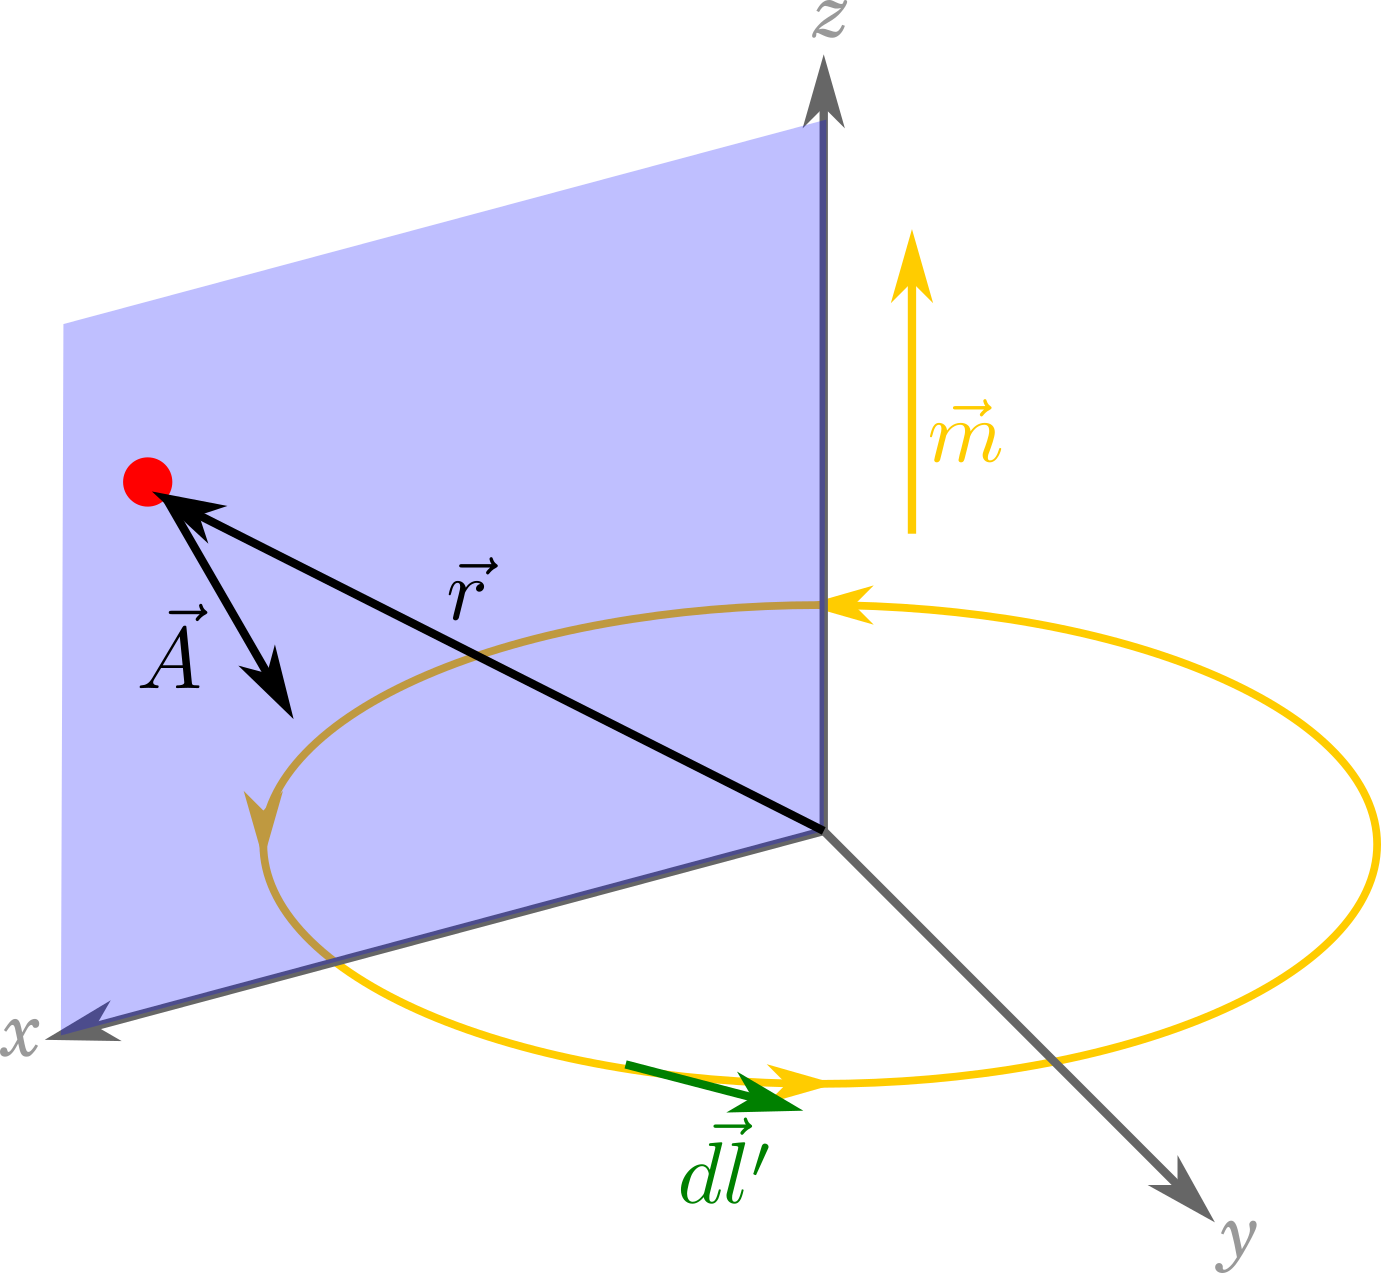
\includegraphics[width=0.7\linewidth]{dip-point-plane-7}
			\label{fig:dip-point-plane-7}
		\end{figure}
		\column[]{0.5\textwidth}
		
		\[ \vec{A}(\vec{r},t) = \mfp \int \dfrac{I_0 \cos \left[\omega \left( t - \rcurs/c \right) \right]}{\rcurs}\, \vec{dl'} \]
		Hence, $ \vec{A} $ has $ \hat{y} $-component only.
		\[ \vec{dl'} = -b\sin\phi'\, d\phi' \, \hat{x} + b\cos\phi'\, d\phi' \, \hat{y} \]
		\[ \therefore \vec{dl'} = b\cos\phi'\, d\phi' \, \hat{y} \]
	\end{columns}
	
\end{frame}

\begin{frame}
	\begin{dmath}\label{eqn : uncooked-A}
		\vec{A} (\vec{r},t) = \mfp \int \dfrac{I_0 \cos\wtRc}{\rcurs}\, \left( b \cos \phi'\, d\phi' \right) \hat{y} \pause
		= \dfrac{\mu_0 I_0 b}{4\pi} \hat{y} \int_{0}^{2\pi} \dfrac{\cos\wtRc}{\rcurs} \cos\phi'\, d\phi' 
	\end{dmath}
\pause	
\begin{columns}
	\column[]{0.25\textwidth}
	\begin{figure}[!htb]
		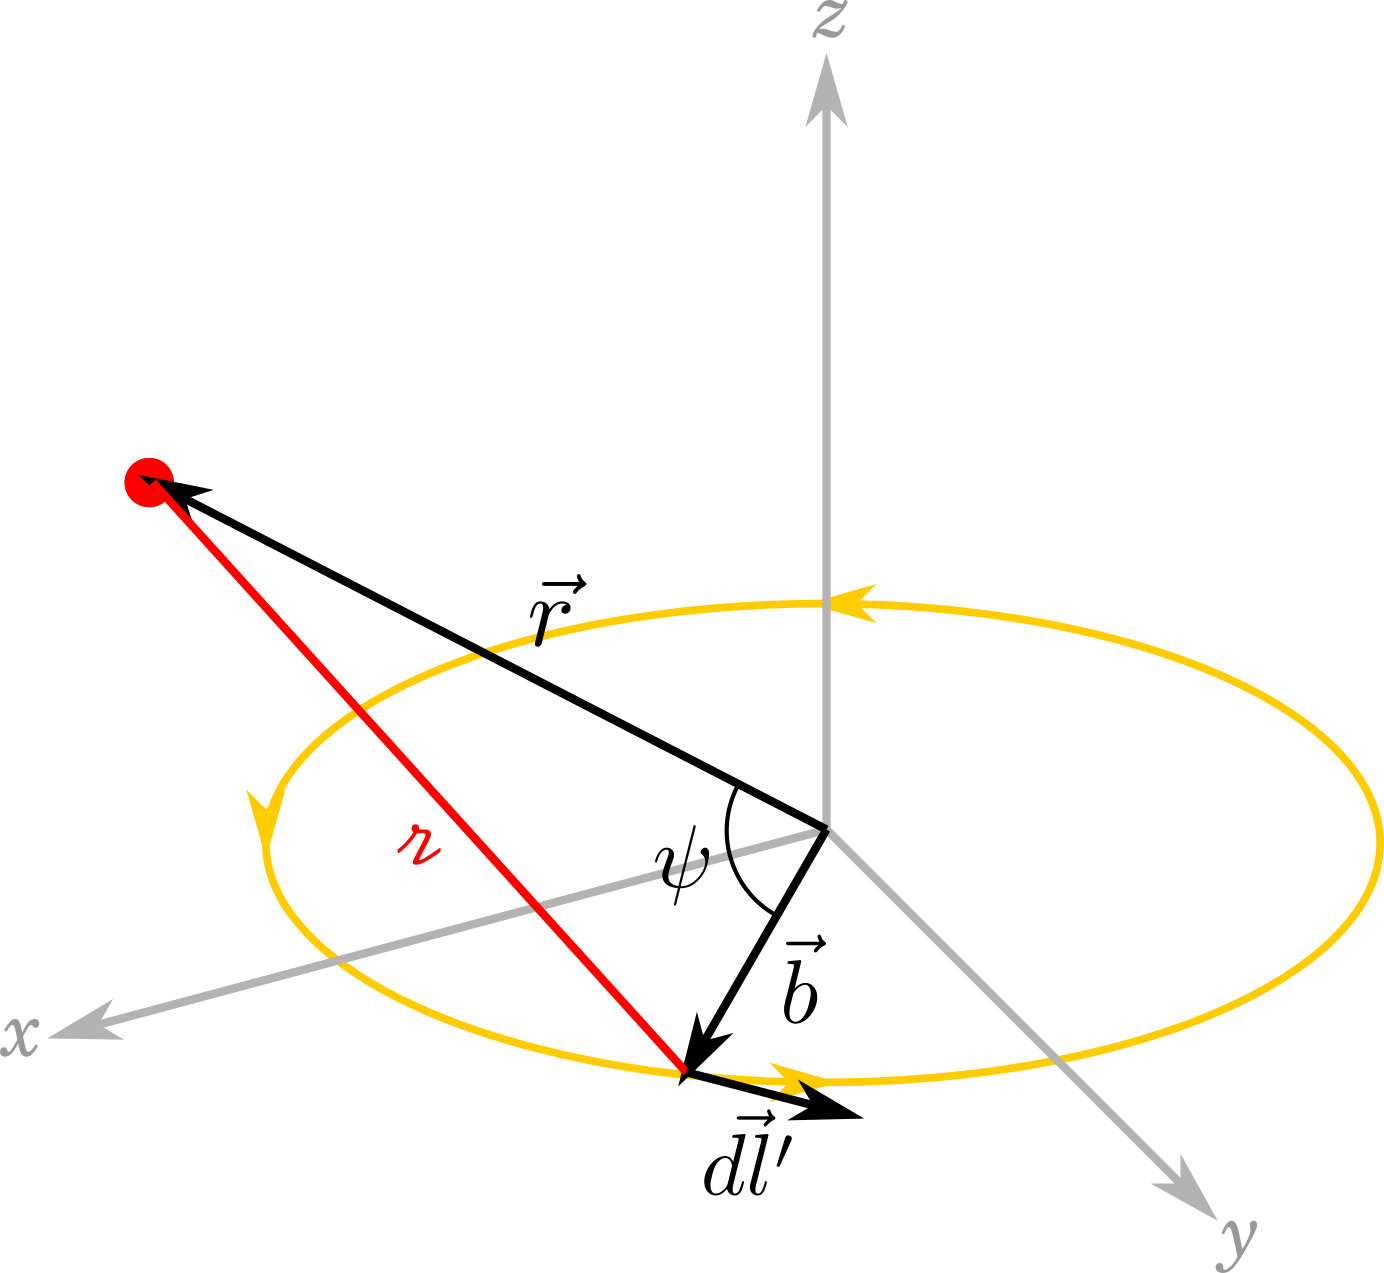
\includegraphics[scale=0.4]{dip-4ps}
	\end{figure}
	\column[]{0.75\textwidth}\pause
	\begin{dmath*}
		\rcurs = \sqrt{ r^2 + b^2 - 2rb \cos\psi} \pause
		= r \sqrt{ 1 + \left( \dfrac{b^2}{r^2} \right) - 2\left(\dfrac{b}{r} \right) \cos\psi}
	\end{dmath*}
	
\end{columns}
\end{frame}	

	\begin{frame}
		\begin{columns}
			\column[]{0.5\textwidth}
			\begin{figure}[!htb]
				\centering
				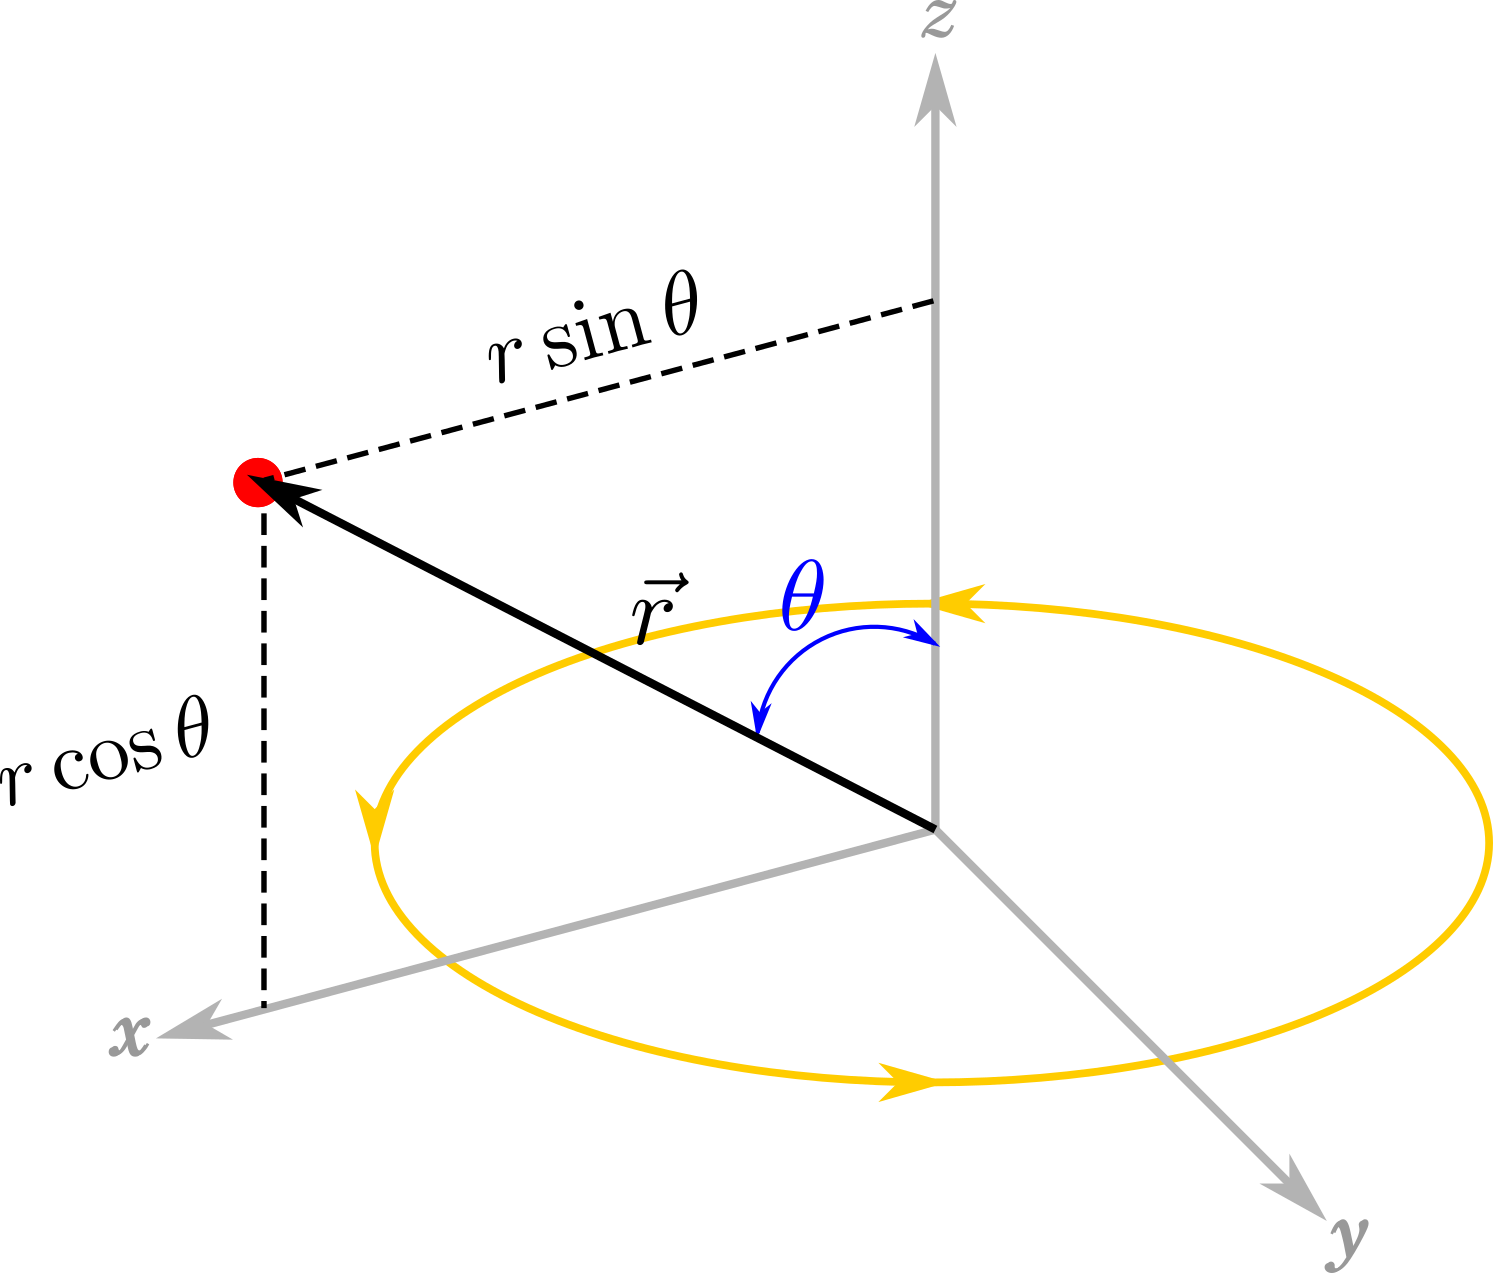
\includegraphics[scale=0.5]{r-components}
			\end{figure}
			\pause
			\[ \vec{r} = r \sin\theta\, \hat{x} + r \cos\theta\, \hat{z} \]
			\pause
			\column[]{0.5\textwidth}
			\begin{figure}[!htb]
				\centering
				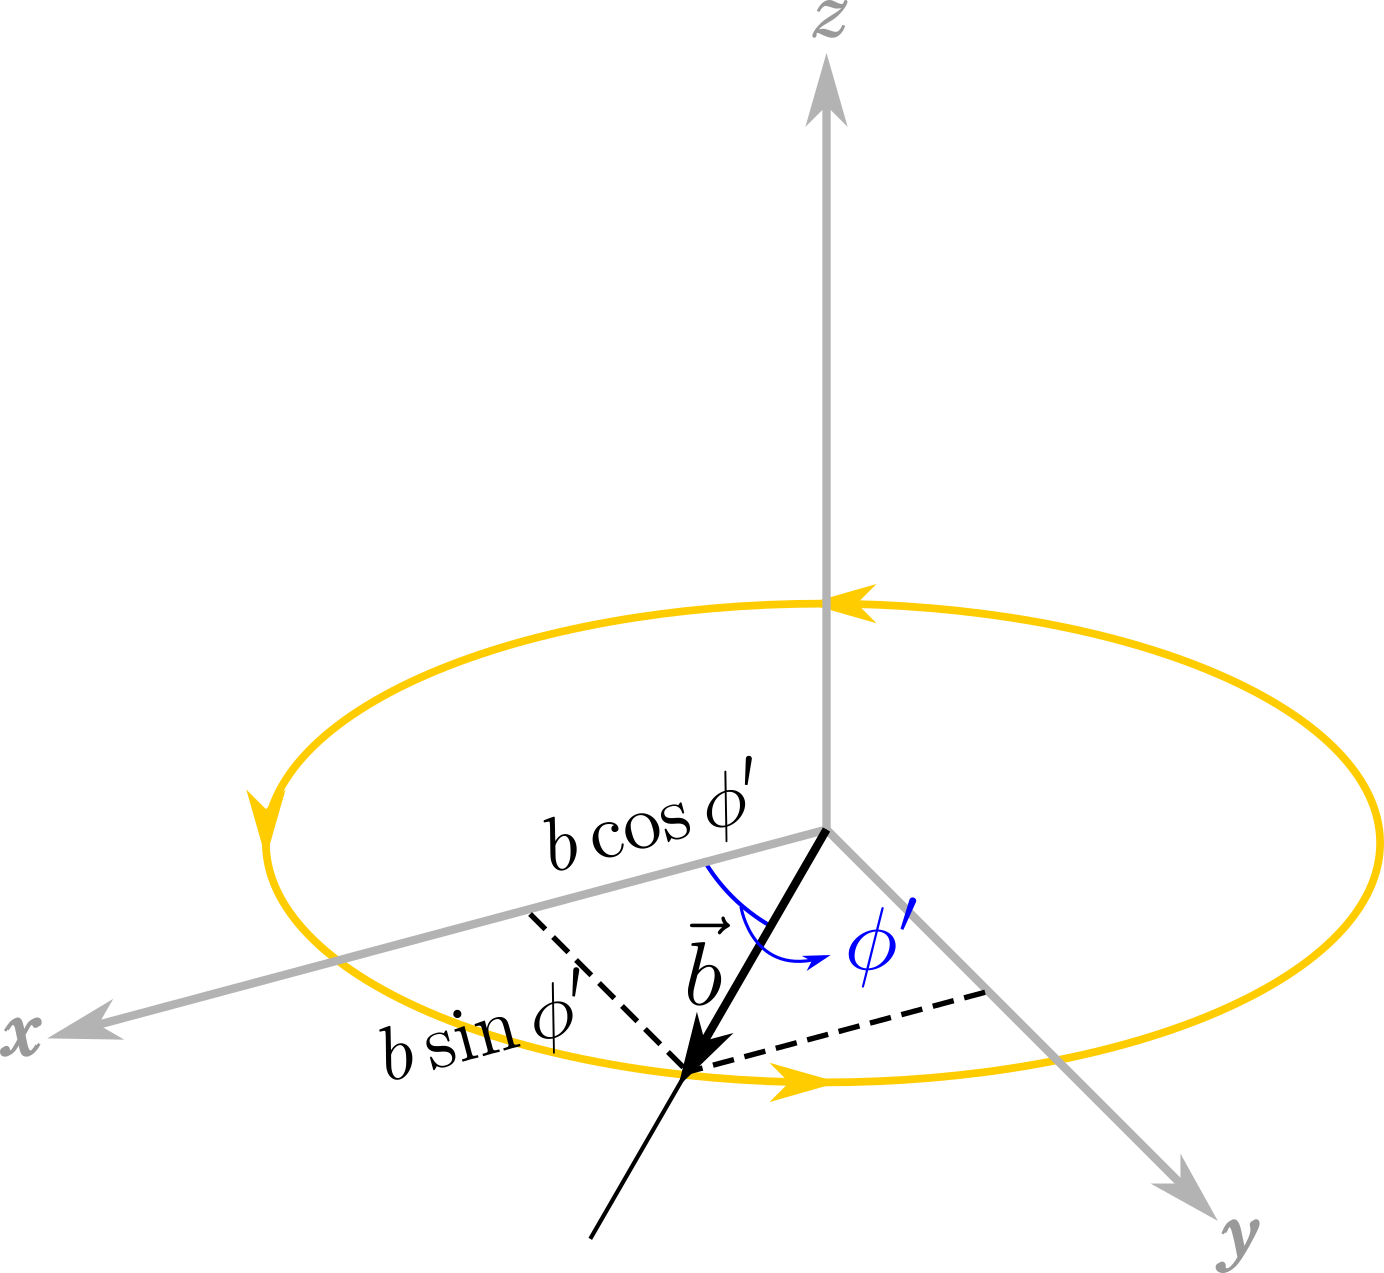
\includegraphics[scale=0.5]{b-components}
			\end{figure}
		\pause
		\[ \vec{b} = b \cos\phi' \hat{x} + b \sin\phi' \hat{y} \]
		
		\end{columns}
	\pause
	\[ \vec{r}\cdot\vec{b} = rb\cos\psi = rb\sin\theta\cos\phi' \]
	\[ \cos\psi = \sin\theta\cos\phi' \]
	\end{frame}

\begin{frame}
	\begin{dmath*}
		\vec{A} (\vec{r},t) = \mfp \int \dfrac{I_0 \cos\wtRc}{\rcurs}\, \left( b \cos \phi'\, d\phi' \right) \hat{y} 
		= \dfrac{\mu_0 I_0 b}{4\pi} \hat{y} \int_{0}^{2\pi} \dfrac{\cos\wtRc}{\rcurs} \cos\phi'\, d\phi'  
	\end{dmath*}
	
	\begin{columns}
		\column[]{0.25\textwidth}
		\begin{figure}[!htb]
			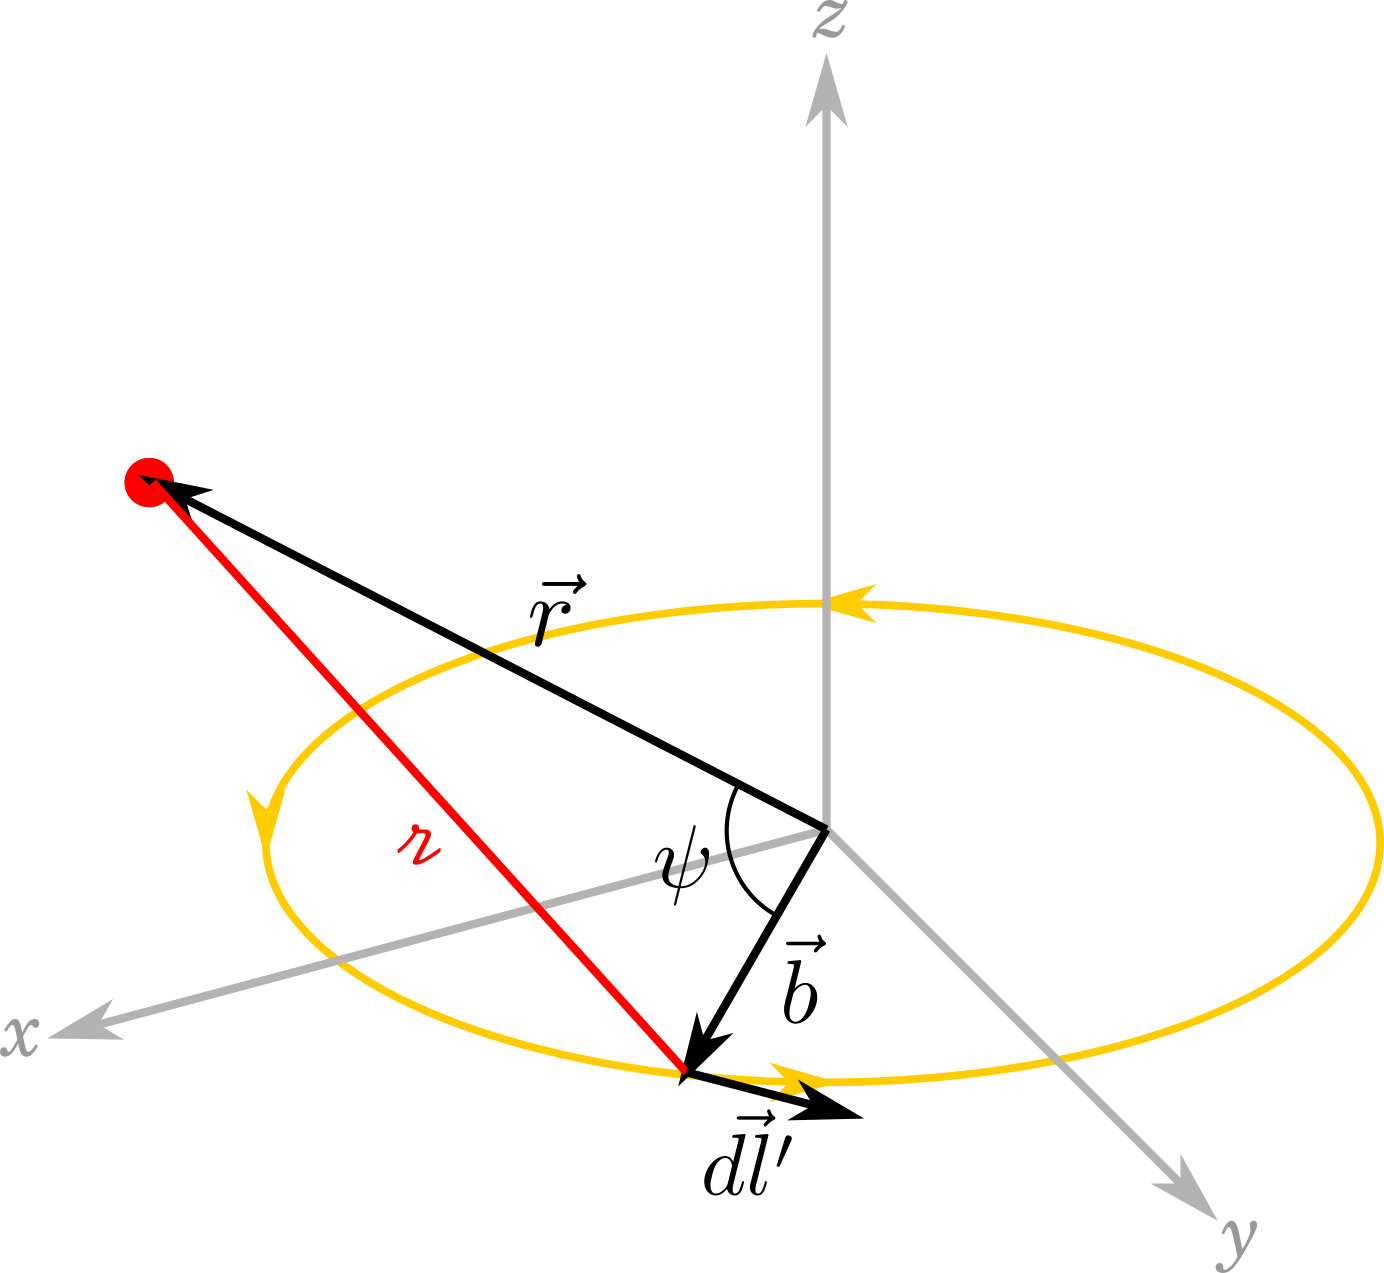
\includegraphics[scale=0.4]{dip-4ps}
		\end{figure}
		\column[]{0.75\textwidth}
		\begin{dmath*}
			\rcurs = \sqrt{ r^2 + b^2 - 2rb \cos\psi} 
			= r \sqrt{ 1 + \left( \dfrac{b^2}{r^2} \right) - 2\left(\dfrac{b}{r} \right) \cos\psi}\pause
			= r \sqrt{ 1 + \left( \dfrac{b^2}{r^2} \right) - 2\left(\dfrac{b}{r} \right) \sin\theta\cos\phi'} \pause
			= r {\left[1 + \left( \dfrac{b^2}{r^2} \right) - 2\left(\dfrac{b}{r} \right) \sin\theta\cos\phi' \right]}^{1/2}
		\end{dmath*}
		
	\end{columns}
\end{frame}		

\begin{frame}
	\begin{columns}
	\column[]{0.5\textwidth}
	\begin{dmath*}
		\rcurs = r {\left[1 + \left( \dfrac{b^2}{r^2} \right) - 2\left(\dfrac{b}{r} \right) \sin\theta\cos\phi' \right]}^{1/2}
	\end{dmath*}
\pause
	\begin{tcolorbox}[width = 5cm]
			\begin{center}
				Approximation 1 : $ b\ll r $
			\end{center}
	\end{tcolorbox}
	\pause
	\begin{dmath*}
		\rcurs = r {\left[1 + \left( \dfrac{b^2}{r^2} \right) - 2\left(\dfrac{b}{r} \right) \sin\theta\cos\phi' \right]}^{1/2} \pause \\
		\approxeq r {\left[1 - 2\left(\dfrac{b}{r} \right) \sin\theta\cos\phi' \right]}^{1/2} \pause \\
		\approxeq r \left[1 - \left(\dfrac{b}{r} \right) \sin\theta\cos\phi' \right] \pause
	\end{dmath*}
	\column[]{0.5\textwidth}
	\begin{dmath*}
		\dfrac{1}{\rcurs} = \dfrac{1}{r} \left[1 - \left(\dfrac{b}{r} \right) \sin\theta\cos\phi' \right]^{-1} \pause \\
		\approxeq \dfrac{1}{r} \left[1 + \left(\dfrac{b}{r} \right) \sin\theta\cos\phi' \right] \pause
	\end{dmath*}
	\begin{equation}\label{eqn : 1/r}
		\boxed{\therefore \dfrac{1}{\rcurs} \approxeq \dfrac{1}{r} \left[1 + \left(\dfrac{b}{r} \right) \sin\theta\cos\phi' \right] } 
	\end{equation}
	\end{columns}
\end{frame}

\begin{frame}
	\begin{dmath*}
		\cos \wtRc =  \pause \cos \Bigg\{ \omega \left[ t - \dfrac{r}{c} \left( 1 - \dfrac{b}{r}\sin\theta\cos\phi' \right) \right] \Bigg\}\pause\\
		=\cos \left[\omega(t-r / c)+\frac{\omega b}{c} \sin \theta \cos \phi^{\prime}\right] \pause \\
		= \cos [\omega(t-r / c)] \cos \left(\frac{\omega b}{c} \sin \theta \cos \phi^{\prime}\right) 
		-\sin [\omega(t-r / c)] \sin \left(\frac{\omega b}{c} \sin \theta \cos \phi^{\prime}\right)\pause 
	\end{dmath*}
\begin{tcolorbox}[width = 7cm]
	\begin{center}
		Approximation 2 : $ b\ll \frac{c}{\omega} $
	\end{center}
\end{tcolorbox}
\pause
\begin{equation}\label{eqn : cos term}
\boxed{\cos [\omega(t-\rcurs / c)] \approxeq \pause \cos [\omega(t-r / c)]-\frac{\omega b}{c} \sin \theta \cos \phi^{\prime} \sin [\omega(t-r / c)]}
\end{equation}
\pause
	\begin{columns}
		\column[]{0.5\textwidth}
		\column[]{0.5\textwidth}
		\footnotesize
		\[ \left(\begin{aligned}
		\cos x &=& 1 - \dfrac{x^2}{2!} + \dfrac{x^4}{4!} - \cdots\\ 
		\sin x &=& x - \dfrac{x^3}{3!} + \dfrac{x^5}{5!} - \cdots 
		\end{aligned}\right) \]
	\end{columns}
\end{frame}

\begin{frame}
	\footnotesize
	Referring to equation (\ref{eqn : uncooked-A})
	\pause
	\[ \vec{A} (\vec{r},t) 
	= \dfrac{\mu_0 I_0 b}{4\pi} \hat{y} \int_{0}^{2\pi} \dfrac{\cos\wtRc}{\rcurs} \cos\phi'\, d\phi'   \]
	\pause
	Substituting equations (\ref{eqn : 1/r}) and (\ref{eqn : cos term}),
	\begin{dmath}
		\vec{A}(\vec{r},t) = \dfrac{\mu_0 I_0 b}{4\pi} \hat{y} \int_{0}^{2\pi}  \Biggl\{ \cos\wtrc - \dfrac{\omega b}{c} \sin\theta\cos\phi' \sin\wtrc \Biggr\}\left(\dfrac{1}{\rcurs}\right)\cos\phi'd\phi'  \pause
		= \dfrac{\mu_0 I_0 b}{4\pi} \hat{y} \int_{0}^{2\pi}  \Biggl\{ \cos\wtrc - \dfrac{\omega b}{c} \sin\theta\cos\phi' \sin\wtrc \Biggr\}\dfrac{1}{r} \left[1 + \left(\dfrac{b}{r} \right) \sin\theta\cos\phi' \right]\cos\phi'd\phi' \pause
		= \dfrac{\mu_0 I_0 b}{4\pi r} \hat{y} \int_{0}^{2\pi}  \Biggl\{ \cos\wtrc - \dfrac{\omega b}{c} \sin\theta\cos\phi' \sin\wtrc \Biggr\} \left[1 + \left(\dfrac{b}{r} \right) \sin\theta\cos\phi' \right]\cos\phi'd\phi' \pause \\
		\approxeq \frac{\mu_{0} I_{0} b}{4 \pi r} \hat{y} \int_{0}^{2 \pi}\left\{\cos [\omega(t-r / c)]+b \sin \theta \cos \phi^{\prime}\left(\frac{1}{r} \cos [\omega(t-r / c)]-\frac{\omega}{c} \sin [\omega(t-r / c)]\right)\right\} \cos \phi^{\prime} d \phi^{\prime} \pause
		= \frac{\mu_{0} I_{0} b}{4 \pi r} \hat{y} \left\{ \int_{0}^{2 \pi}\cos [\omega(t-r / c)] \cos \phi^{\prime} d \phi^{\prime} + \int_{0}^{2 \pi} b \sin \theta \cos^2 \phi^{\prime} \left(\frac{1}{r}\cos [\omega(t-r / c)] - \frac{\omega}{c} \sin [\omega(t-r / c)]\right) d\phi' \right\}
	\end{dmath}
\end{frame}

\begin{frame}
	\small
	\begin{dmath*}
		\vec{A}(\vec{r},t) = \frac{\mu_{0} I_{0} b}{4 \pi r} \hat{y} \left\{ \int_{0}^{2 \pi}\cos [\omega(t-r / c)] \color{high}\cos \phi^{\prime} d \phi^{\prime} \color{black} + \int_{0}^{2 \pi} b \sin \theta \color{high} \cos^2 \phi^{\prime} \color{black}\left(\frac{1}{r}\cos [\omega(t-r / c)] - \frac{\omega}{c} \sin [\omega(t-r / c)]\right) \color{high}d\phi' \color{black}\right\}
	\end{dmath*}
		\pause
		\[ \int_{0}^{2\pi} \cos \phi' d\phi' = 0 \quad\qquad 	\int_{0}^{2\pi} \cos^2 \phi' d\phi' = \pi  \] \pause
	\begin{dmath*}
		\vec{A}(\vec{r},t) = \frac{\mu_{0} I_{0} b}{4 \pi r} \hat{y} \left\{ 0 + b \sin \theta \color{high} (\pi) \color{black}\left(\frac{1}{r}\cos [\omega(t-r / c)] - \frac{\omega}{c} \sin [\omega(t-r / c)]\right) \color{black}\right\}\pause
		= \frac{\mu_{0} (I_{0} \pi b^2)}{4 \pi r}  \sin \theta \left(\frac{1}{r}\cos [\omega(t-r / c)] - \frac{\omega}{c} \sin [\omega(t-r / c)]\right) \color{black}\, \hat{y}
	\end{dmath*}
	\pause
	\begin{tcolorbox}
		\begin{equation}\label{eqn : finally}
		\vec{A}(r, \theta, t)=\frac{\mu_{0} m_{0}}{4 \pi}\left(\frac{\sin \theta}{r}\right)\left\{\frac{1}{r} \cos [\omega(t-r / c)]-\frac{\omega}{c} \sin [\omega(t-r / c)]\right\} \hat{\phi}
		\end{equation}
	\end{tcolorbox}
\end{frame}

\begin{frame}
	In the radiation zone, we can make a third approximation:\pause
	\begin{tcolorbox}[width = 6cm]
		\begin{center}
			Approximation 3 : $ r \gg \dfrac{c}{\omega} $
		\end{center}
	\end{tcolorbox}
	\pause
	\begin{tcolorbox}[colframe = amber, colback = amber!20]
		\begin{equation}\label{eqn : FINALLYY}
		\vec{A}(r, \theta, t)=-\frac{\mu_{0} m_{0} \omega}{4 \pi c}\left(\frac{\sin \theta}{r}\right) \sin [\omega(t-r / c)] \hat{\phi}
		\end{equation}
	\end{tcolorbox}
\end{frame}

\begin{frame}[standout]
		The retarded potentials of an oscillating magnetic dipole are:\pause
		\[ \alert{V = 0}\]\pause
		and
		\[ \alert{\vec{A}(r, \theta, t)=-\frac{\mu_{0} m_{0} \omega}{4 \pi c}\left(\frac{\sin \theta}{r}\right) \sin [\omega(t-r / c)] \hat{\phi}} \]
\end{frame}

\begin{frame}{Remarks}
	\footnotesize
	\begin{itemize}
		\item 		The corresponding fields due to these retarded potentials are:\pause
		\begin{equation}\label{eqn : E}
			\vec{E}=-\frac{\partial \vec{A}}{\partial t}=\frac{\mu_{0} m_{0} \omega^{2}}{4 \pi c}\left(\frac{\sin \theta}{r}\right) \cos [\omega(t-r / c)]\, \hat{\phi}
		\end{equation}\pause
			\begin{equation}\label{eqn : B}
			\vec{B}=\vec{\nabla} \times \vec{A}=-\frac{\mu_{0} m_{0} \omega^{2}}{4 \pi c^{2}}\left(\frac{\sin \theta}{r}\right) \cos [\omega(t-r / c)]\, \hat{\theta}
		\end{equation}
		\pause
		
		\begin{figure}
			\centering
			\fbox{\includegraphics[width=0.7\linewidth]{"Mag dip radn - Electromagnetism - Tamer"}}
			\label{fig:mag-dip-radn---electromagnetism---tamer}
		\end{figure}\pause
		
		\item 	These fields are in phase, mutually perpendicular, and transverse to the direction of propagation $ \left(\hat{r}\right) $, and the ratio of their amplitudes is $E_0 / B_0 = c$, all of which is as expected for electromagnetic waves.
		
	\end{itemize}
\end{frame}

\begin{frame}{References}
	\begin{enumerate}
		\item 		David J. Griffiths, \emph{Introduction To
			Electrodynamics}, Fourth Edition
		
		\item 		Tamer B{\'e}cherrawy, \emph{Electromagnetism : Maxwell's Equations, Wave Propagation and Emission}
	\end{enumerate}
\end{frame}

\end{document}